\chapter{Facilitating the Development of Gesture-based Applications} \label{chap:quantumleap}

The landscape of contactless UIs is constantly evolving. Sensors such as the LMC are paving the way towards cheap and accurate gesture recognition, while researchers are continuously working on improving gesture recognition algorithms.
However, the lack of a common framework for gesture recognition is making it increasingly harder to keep track of this evolution outside of the research community, resulting in only a handful of real-life applications (see Sections~\ref{sec:state_of_the_art:overview:applications} and \ref{sec:state_of_the_art:lmc}). 
%
As such, this chapter attempts to answer two of the five research questions defined in Section~\ref{sec:introduction:research:research-questions}: 
\begin{itemize}
    \item [RQ4] \textit{How can we foster collaboration between researchers and practitioners working on (radar) gesture recognition?} 
    \item [RQ5] \textit{How can tools and methods aid in designing gesture-based applications that operate independently of gesture recognition logic?}
\end{itemize}
To that end, it introduces \ql, a software tool that aims at bridging the gap between researchers and developers by providing a common framework to (1) help researchers share the results of their work in a way that is easily reusable and (2) allow developers to create gesture-based applications without spending time to solve the numerous challenges of gesture recognition (see Section~\ref{sec:state_of_the_art:overview:challenges}). The main contribution of this chapter and how it fits into the rest of this thesis are summarized in \fig~\ref{fig:quantumleap:graphical-summary}.

\begin{figure}
    \centering
    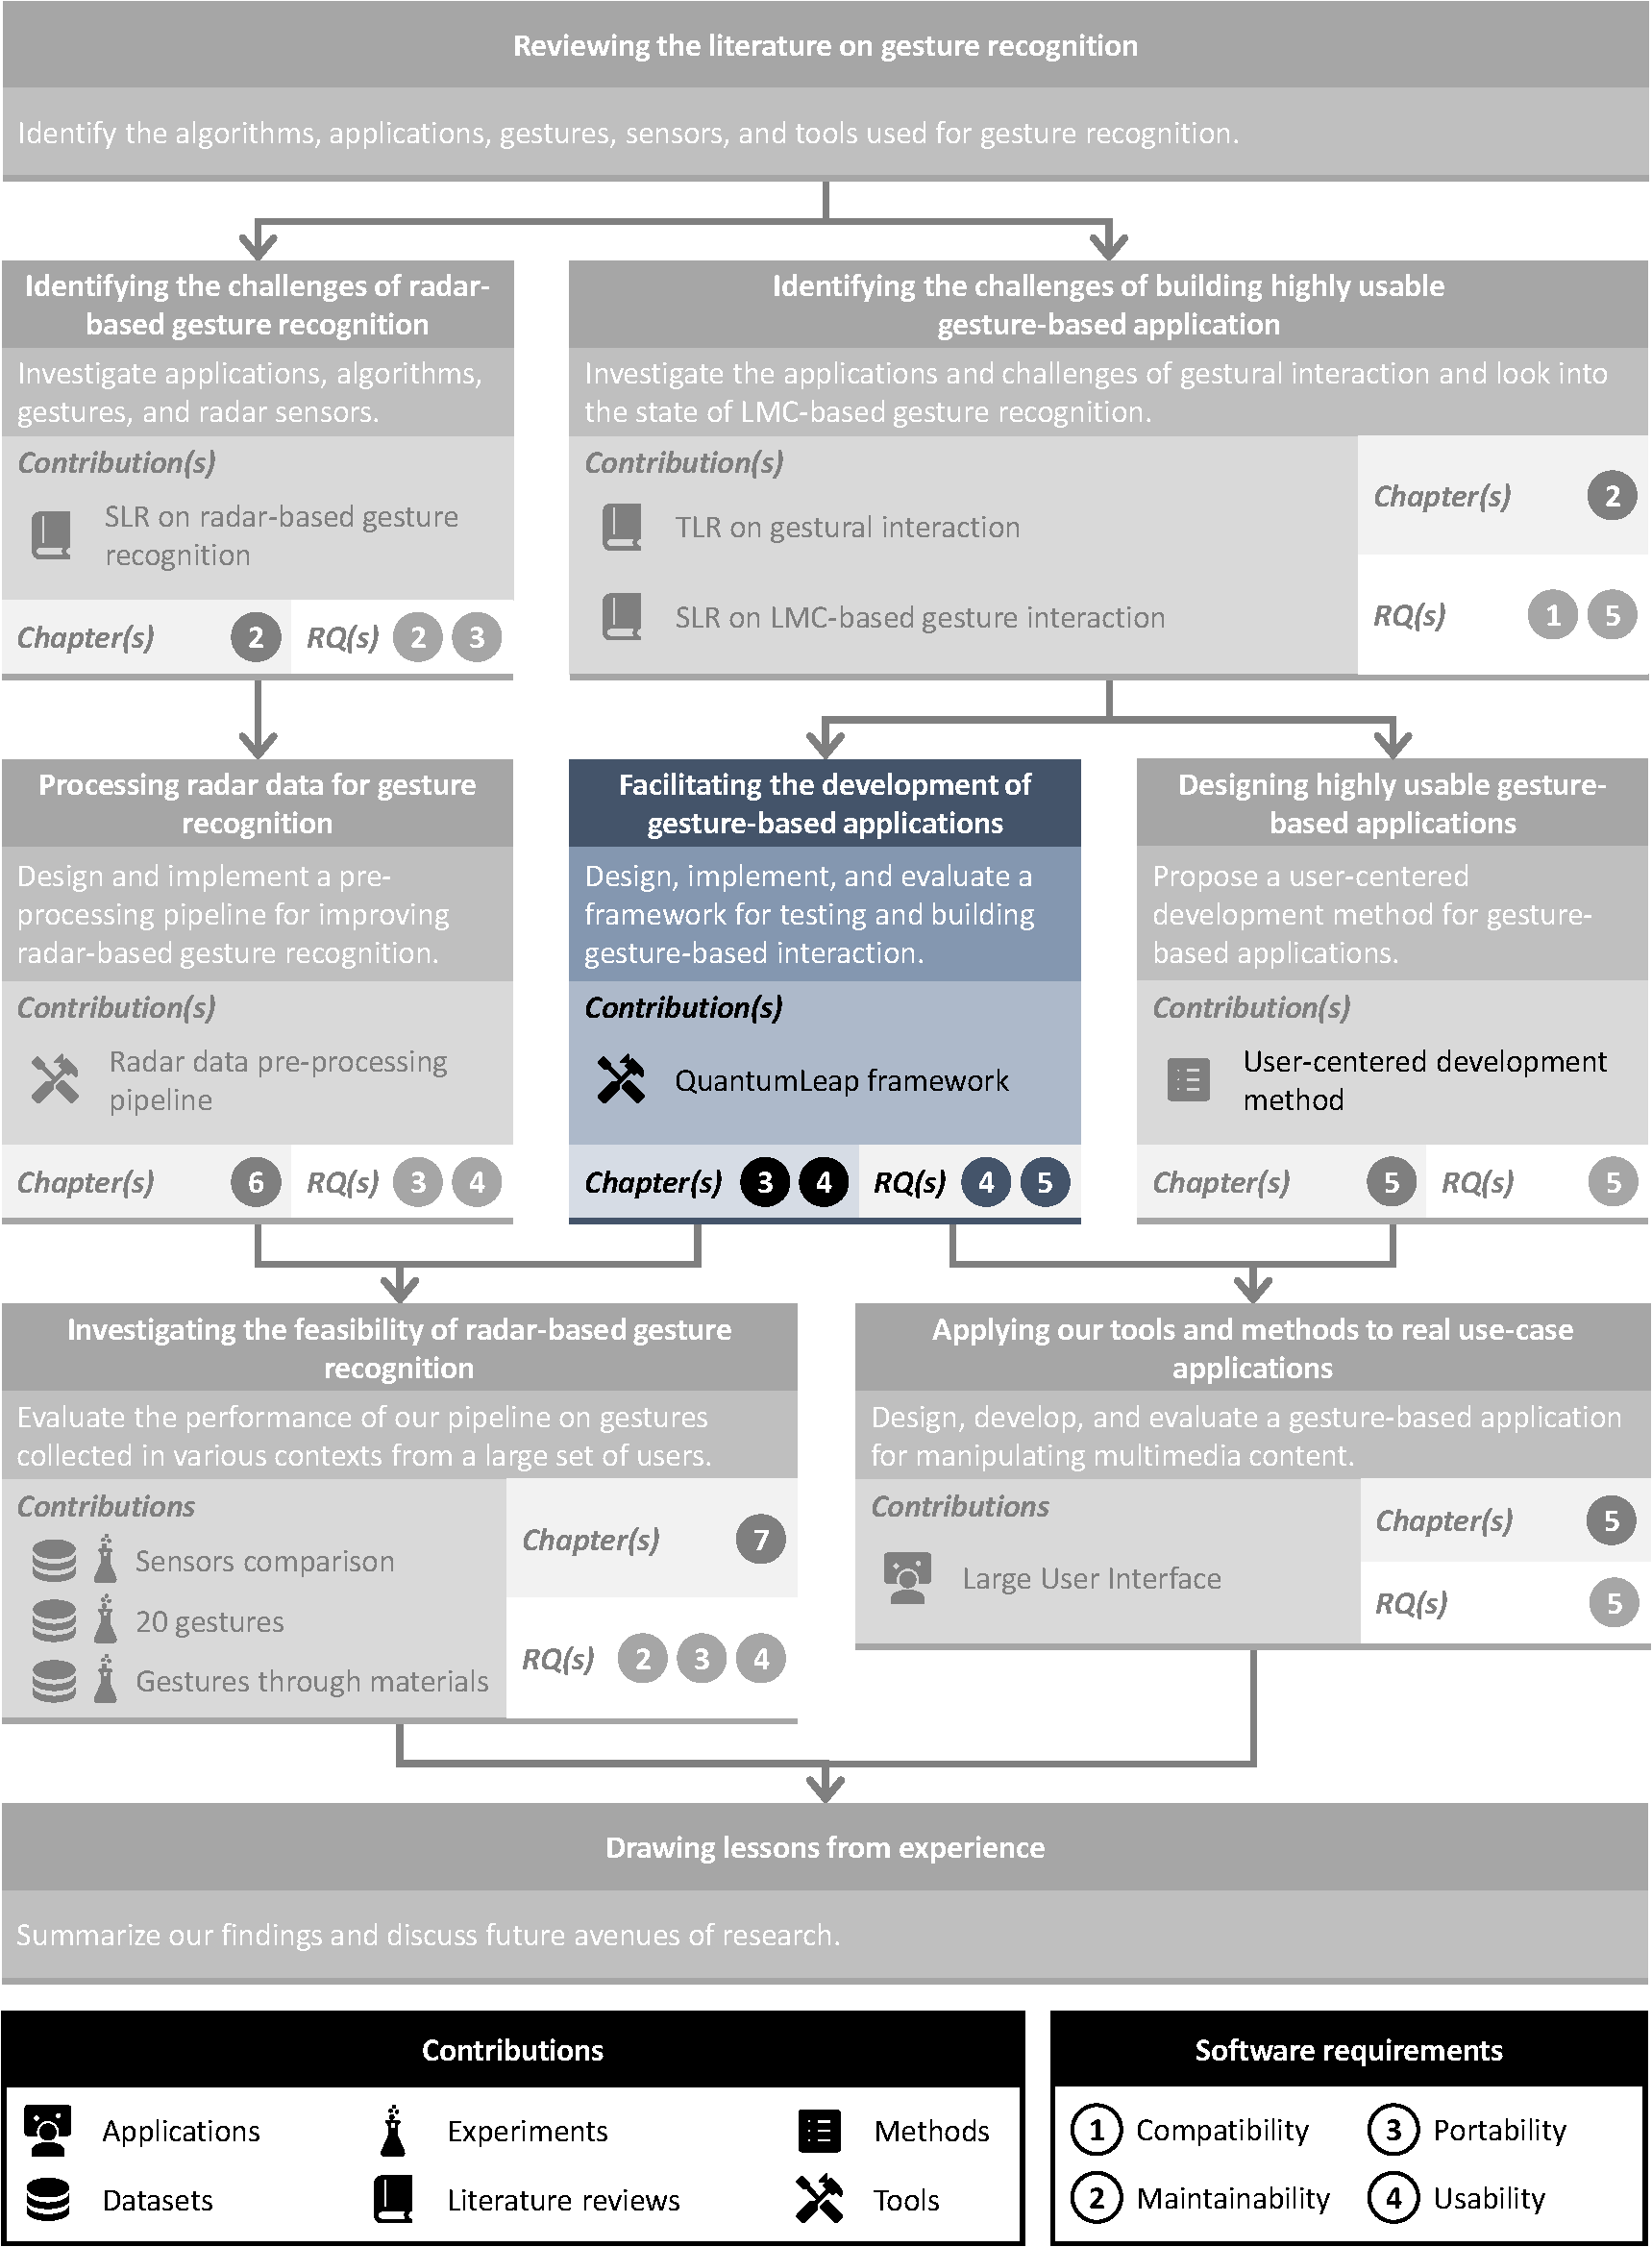
\includegraphics[width=\linewidth]{Figures/QuantumLeap/graphical-summary-quantumleap.pdf}
    \vspace{-18pt}
    \caption{Main contributions of this chapter.}
    \label{fig:quantumleap:graphical-summary}
\end{figure}

The rest of this chapter is organized as follows. Section~\ref{sec:quantumleap:description} first provides an in-depth description of \ql, including its dataflow architecture, configuration, and API.
Section~\ref{sec:quantumleap:evaluation} discusses the results of an experiment aimed at evaluating the overall usability of \ql, which involved seven developers with different levels of expertise.
Section~\ref{sec:quantumleap:integration} then explores how some recent projects utilized and extended the framework.
Finally, Section~\ref{sec:quantumleap:discussion} discusses the advantages and limitations of \ql, and Section~\ref{sec:quantumleap:conclusion} concludes this chapter.

\paragraph{Publications.} This chapter is adapted from a paper published in the EICS 2022 conference proceedings~\cite{Sluyters:2022:EICS}.

\paragraph{Resources.} The \ql framework is available on GitHub at \url{https://github.com/sluyters/QuantumLeap}. Demonstration videos of applications built with \ql are available at \url{https://www.youtube.com/playlist?list=PLj1KcEqIa0fHyDyeW_NpiLHCP6A8j7mS3}.


%================================================================================%
\section{A Framework for Building Gesture-Based Applications} \label{sec:quantumleap:description}

\ql is designed as an intermediate layer between gesture-based applications and gesture sensors. It contains all of the logic necessary for gesture recognition and only exposes a simple JavaScript API that allows developers to map gestures to actions without focusing on acquiring, segmenting, and recognizing gestures. 
Implemented in JavaScript (ECMAScript 2019)~\cite{Ecma:2017}, the \ql framework is divided into two parts according to Pree's notation \cite{Pree:1994}: \textit{frozen spots}, which are ``fixed'' parts which remain constant for all of its instantiations, and \textit{hot spots}, which are generic parts to be modified depending on the context of use~\cite{Calvary:2003}.
\ql is a \textit{gray box} software framework~\cite{Parsons:1999}, as it provides developers with two options: pick modules from a list of predefined components (black box) or write new components that meet their needs better (white box).
The rest of this section describes the overall software architecture of \ql.
%, its API, and how it can be configured for a specific context of use.

%--------------------------------------------------------------------------------%
\subsection{Dataflow Architecture} \label{sec:quantumleap:description:architecture}

The dataflow architecture of \ql (\fig~\ref{fig:quantumleap:archi}) has been designed to be versatile and simple to configure (Section~\ref{sec:quantumleap:description:configuration}). It consists of eight modules (\ie hot spots), each stemming from the challenges of gesture recognition discussed in Section~\ref{sec:state_of_the_art:overview:challenges}: a sensor module, filtering module, loaders for static and dynamic datasets, static and dynamic gesture recognizers, gesture segmentation module, and an analyzer module. Various implementations are provided for each module to suit the needs of a specific application (see Appendix~\ref{app:quantumleap-modules}). When these implementations are not suited for a particular application, the framework is extensible and developers are thus encouraged to propose new implementations. The modules communicate together using various data structures described in \tab~\ref{tbl:quantumleap:communication-data-structures}. 
The rest of this section provides information about each type of module.

\begin{table}[t]
    \footnotesize
    \centering
    \begin{tabular}{lp{10.8cm}}
        \toprule
        \textbf{Id} & \textbf{Description} \\
        \midrule
        1 & \custominlinecode{Frame} object. \\
        2 & \custominlinecode{Sample} object. \\
        3 & JavaScript object with three properties: the gesture type (\ie static or dynamic), the gesture name, and the data from the analyzer if the gesture is static. \\
        4 & WebSocket message of type \custominlinecode{Data} containing frames and static\slash dynamic gestures if detected. \\
        5 & WebSocket message of type \custominlinecode{Operation}. \\
        \bottomrule
    \end{tabular}
    \caption{Data structures for inter-module communication.}
    % \vspace{-18pt}
    \label{tbl:quantumleap:communication-data-structures}
\end{table}



\begin{figure}[t]
    \centering
    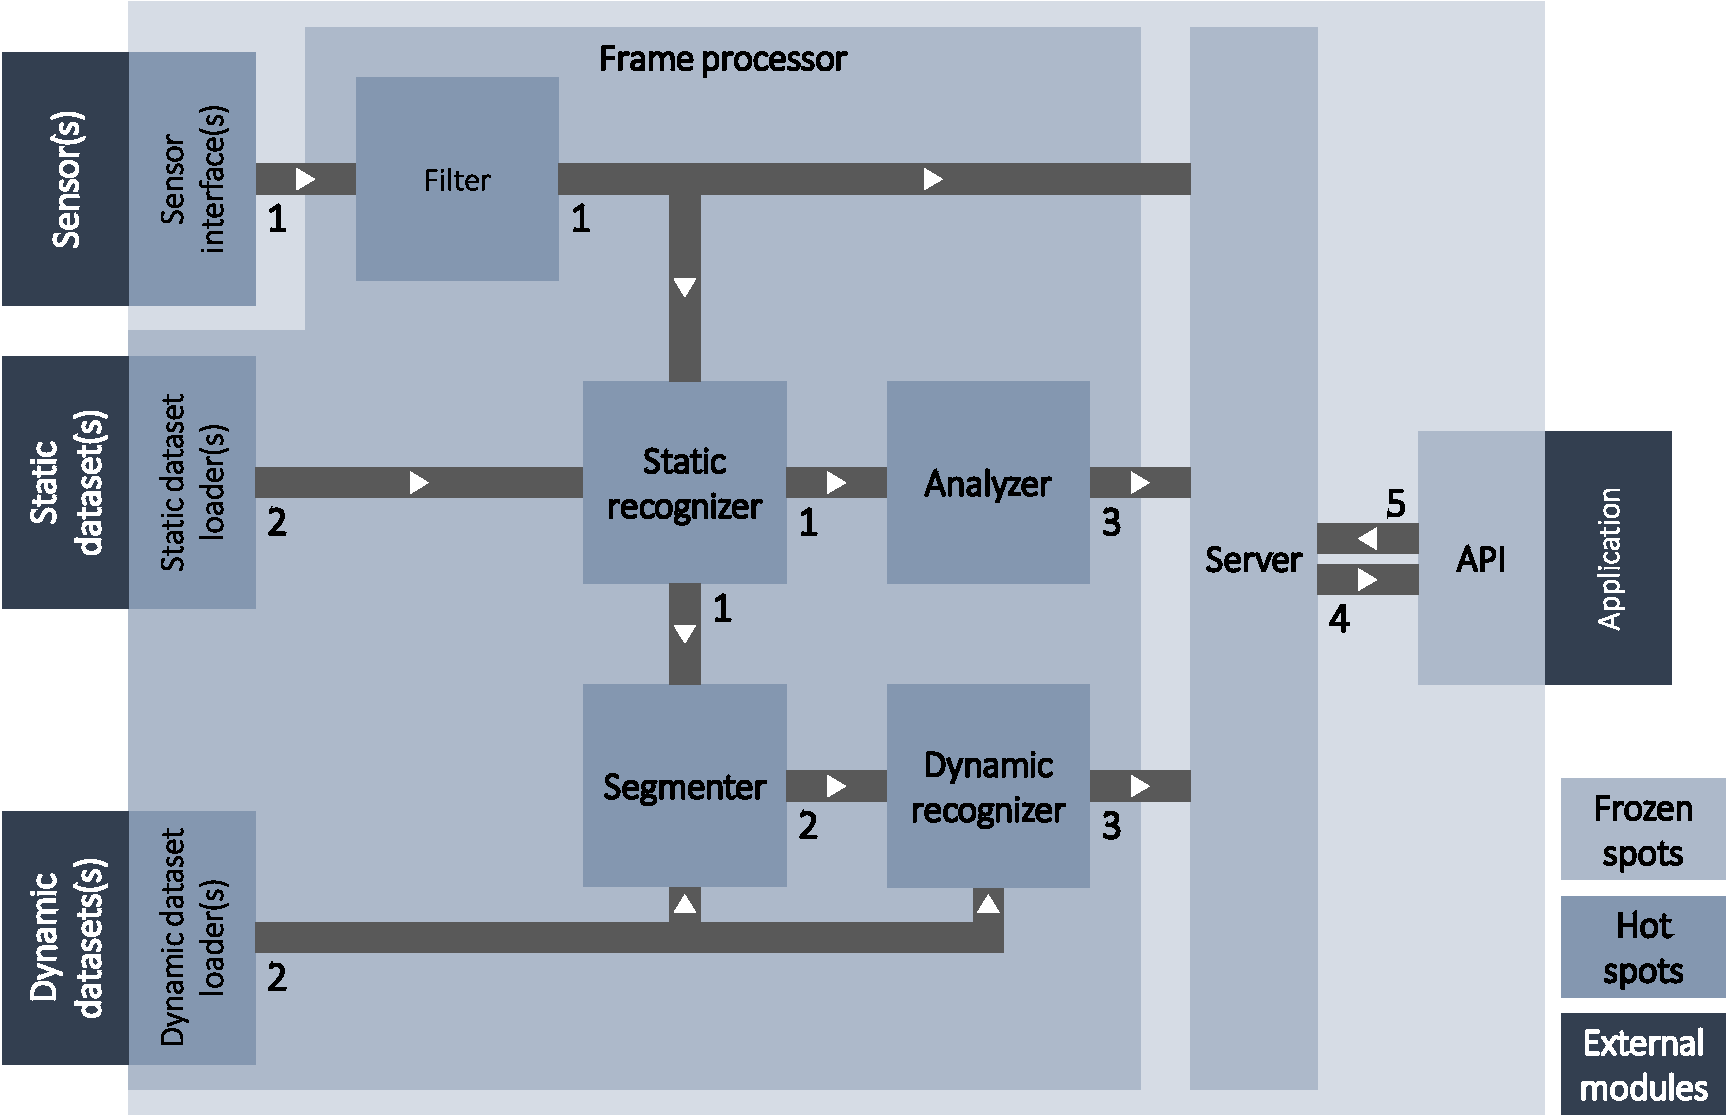
\includegraphics[width=\linewidth]{Figures/QuantumLeap/Architecture/quantumleap.pdf}
    \vspace{-8pt}
    \caption{\ql dataflow architecture.}
    % \vspace{-8pt}
    \label{fig:quantumleap:archi}
\end{figure}

\subsubsection{Sensor} 
This module serves as an interface between \ql and any physical sensor, such as an LMC, a radar sensor, or a Microsoft Kinect. It transforms raw, sensor-specific data into a standardized format usable throughout the framework. This module is called a set number of times per second by \ql to retrieve tracking data at one instant in time. Depending on the context of use, multiple sensor modules may be combined, \eg to increase recognition accuracy. A sensor module should implement three methods:
\begin{itemize}[noitemsep]
    \item \custominlinecode{getPoints(timestamp)}: get a list of points from the sensor at this instant in time.
    \item \custominlinecode{connect()}: connect to the sensor.
    \item \custominlinecode{disconnect()}: disconnect from the sensor.
\end{itemize}
One sensor module is provided with \ql. Its description can be found in Appendix~\ref{app:quantumleap-modules:sensors}.

\subsubsection{Filter}
As discussed in Section~\ref{sec:noise}, noise can negatively impact the user experience by reducing pointing and gesture recognition accuracy. Before it can be used by the other modules, each frame is first processed by the filter module, which computes a new frame with reduced noise. Filtering should be carefully tuned to fit the sensor and the target application, as too much noise reduction runs the risk of introducing some lag. A filter module should implement one method:
\begin{itemize}[noitemsep]
    \item \custominlinecode{filter(frame)}: compute a new frame with less noise.
\end{itemize}
Four different modules are provided and described in Appendix~\ref{app:quantumleap-modules:filters}.

\subsubsection{Static and Dynamic Datasets}
These modules transform a gesture dataset into a \custominlinecode{GestureSet} object, \ie a standardized format compatible with the framework. Datasets are then used to train the static and dynamic recognizers.
\begin{figure*}[p]
    \centering
    % \vspace{-6pt}
    \captionsetup{justification=centering}
    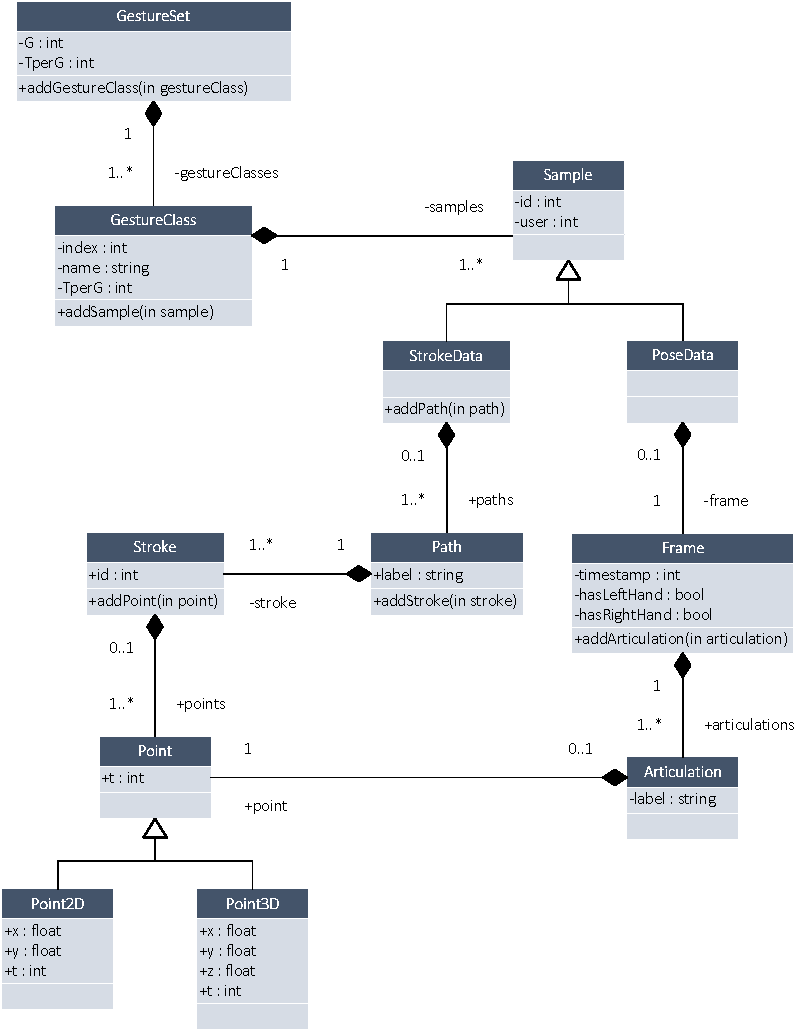
\includegraphics[width=\linewidth]{Figures/QuantumLeap/Architecture/QuantumLeap-UML.pdf}
    % \vspace{-4pt}
    \caption{UML V2.5 class diagram of the gesture sets.}
    \label{fig:quantumleap:dataset-uml}
    % \vspace{-12pt}
\end{figure*}
\fig~\ref{fig:quantumleap:dataset-uml} depicts the UML V2.5 \cite{Bush:2011} Class diagram of the modular data structure used in the framework. The \custominlinecode{GestureSet} object can contain samples of two types: (1) \custominlinecode{PoseData}, for static gestures consisting of a single frame that represents a hand pose; and (2) \custominlinecode{StrokeData}, for dynamic gestures, which comprise multiple paths, where a path corresponds to the trajectory~\cite{Caputo:2018} of a specific joint (\eg the tip of the right index). Paths are in turn decomposed into a series of strokes. Only one method is required:
\begin{itemize}[noitemsep]
    \item \custominlinecode{loadDataset(name, path, identifier)}: load a gesture dataset into memory as a \custominlinecode{GestureSet} object.
\end{itemize}
Developers have two possibilities for selecting a gesture set. They can create a custom gesture set with any specialized software, such as \textsc{Magic2}~\cite{Kohlsdorf:2011} or \textsc{GestMan}~\cite{Magrofuoco:2019a}, or via an LMC gesture recorder\footnote{We release the code of the LMC Gesture Recorder on GitHub at \url{https://github.com/sluyters/LeapGesturePlayback}.}. Another option is to pick one of the many publicly available datasets, such as SHREC2019~\cite{Caputo:2019}, and convert it into the standardized format to be considered in \ql.

\subsubsection{Static Recognizer}
The static recognizer module attempts to recognize static gestures at each frame. For each recognized gesture, the recognizer should compute a confidence score ranging from 0 to 1, where 1 indicates that it is absolutely confident that it has correctly identified the gesture. If the score is lower than a manually set threshold, the gesture is rejected. In the future, this threshold could be automatically computed by \ql for each gesture class based on the training dataset(s). Having a dedicated module for static gesture recognition allows using more efficient recognizers that are specialized for this task. This should thus result in increased accuracy and lower CPU usage. A static recognizer module should implement three methods:
\begin{itemize}[noitemsep]
    \item \custominlinecode{addGesture(name, frame)}: add a static gesture to the training set of this recognizer.
    \item \custominlinecode{removeGesture(name)}: remove a static gesture from the training set of this recognizer (including all of its samples).
    \item \custominlinecode{recognize(frame)}: determine the name of the static gesture performed in the frame given as argument.
\end{itemize}
To avoid accidentally triggering dynamic gestures while the user is performing a static gesture, the recognition of dynamic gestures is stopped when a static gesture is recognized. Two static recognizer modules are provided and described in Appendix~\ref{app:quantumleap-modules:static-recognizers}.

\subsubsection{Analyzer}
These modules extract additional data from the sensor frames, which can then be used inside applications. They can serve to offload heavy computation from the front-end to the \ql dataflow, to implement more advanced feature extraction techniques that would otherwise clutter the front-end application, or to remove sensor-dependent code from the application. Any analyzer module should implement two methods:
\begin{itemize}[noitemsep]
    \item \custominlinecode{analyze(frame)}: extract relevant information from a frame.
    \item \custominlinecode{reset()}: reset the internal state of the analyzer.
\end{itemize}
As analyzer modules are highly specific to the application, we expect developers to create their own modules. However, one simple module is provided and described in Appendix~\ref{app:quantumleap-modules:analyzers}.

\subsubsection{Segmenter}
The role of this module is to identify intentional dynamic gestures from a continuous stream of data. It analyzes frames one by one until it identifies a gesture. It then returns one or more lists of frames (\eg if it has multiple sliding windows), which are subsequently transformed into \custominlinecode{StrokeData} objects that are sent to the dynamic gesture recognizer for recognition. If multiple lists of frames are returned at the same time, only the gesture with the highest confidence score is kept.
The most appropriate method for gesture segmentation varies depending on the application, environment, and sensor(s). For instance, a simple sliding window segmenter could be appropriate for a multimedia application, while a more accurate technique may be required in environments where mistakes are costly, such as operating rooms. It is thus important to leave the choice of segmenter to the designer. A segmenter module should implement four methods:
\begin{itemize}[noitemsep]
    \item \custominlinecode{addGesture(name, sample)}: add a dynamic gesture to the training set of the segmenter.
    \item \custominlinecode{removeGesture(name)}: remove a dynamic gesture from the training set of the segmenter (including all of its samples).
    \item \custominlinecode{computeSegments(frame)}: process a frame and return one or more lists of frames (\ie segments) if the frame marks the ending of a gesture.
    \item \custominlinecode{notifyRecognition()}: notify the segmenter that a gesture has been recognized. The segmenter may use this information to take the coarticulation between two subsequent gestures into account (\eg by temporarily pausing gesture segmentation after a gesture is recognized).
\end{itemize}
Three different segmenters are provided and described in Appendix~\ref{app:quantumleap-modules:segmenters}.

\subsubsection{Dynamic Recognizer}
Distinct from the static recognizers, dynamic recognizers analyze sequences of frames instead of individual frames. They are thus called only when the segmenter detects an intended gesture, which limits CPU usage and reduces the number of false positives. As for the static recognizers, they should return a confidence score for each recognized gesture and implement three methods:
\begin{itemize}[noitemsep]
    \item \custominlinecode{addGesture(name, sample)}: add a gesture to the training set of this recognizer. 
    \item \custominlinecode{removeGesture(name)}: remove a gesture from the training set of this recognizer (including all of its samples).
    \item \custominlinecode{recognize(sample)}: determine the name of the gesture that corresponds to the candidate sample given as argument.
\end{itemize}
Ten dynamic recognizers are provided that cover multiple properties of gesture sets, such as uni- \vs multi-stroke and properties of invariance (see Appendix~\ref{app:quantumleap-modules:dynamic-recognizers}).

%--------------------------------------------------------------------------------%
\subsection{Configuration} \label{sec:quantumleap:description:configuration}

\begin{figure}[!b]
    \centering
    \begin{subfigure}{.49\textwidth}
        \centering
        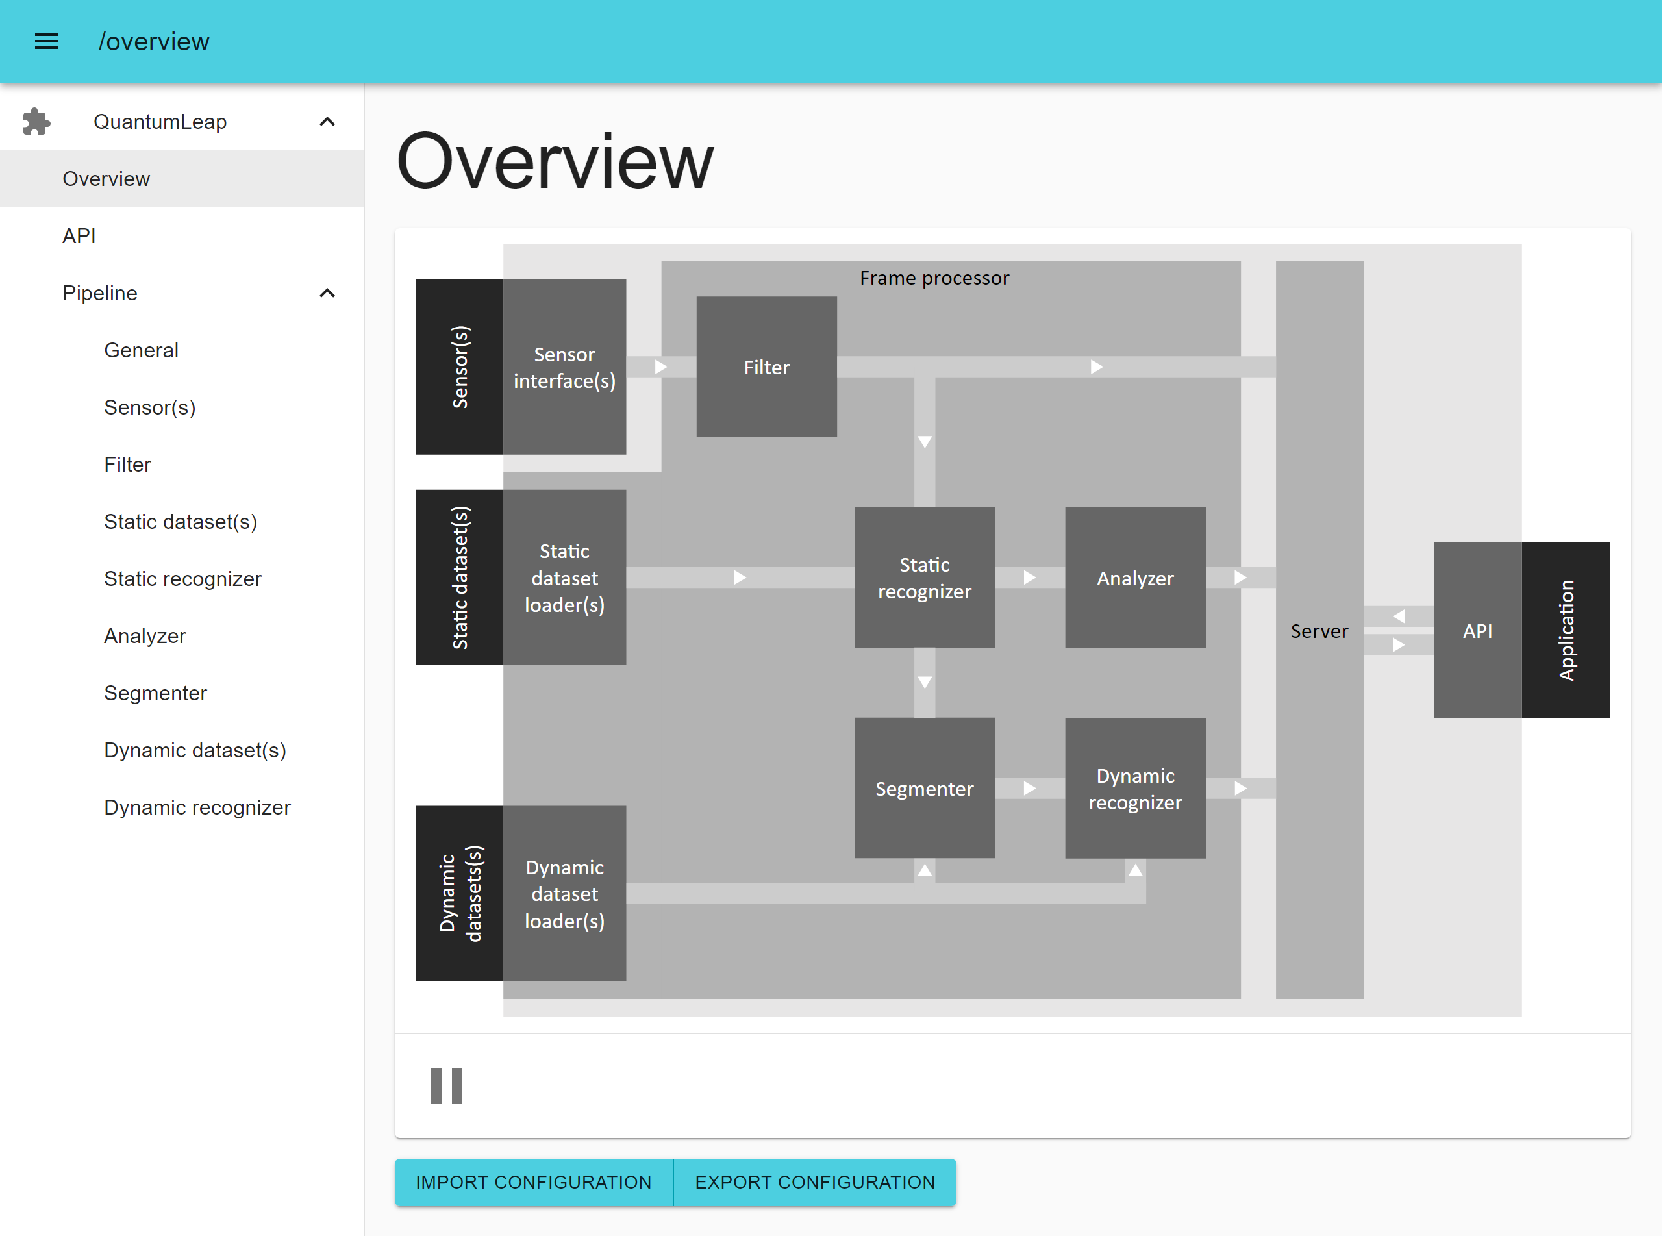
\includegraphics[width=\linewidth]{Figures/QuantumLeap/UI/overview.pdf}  
        \vspace{-15pt}
        \captionsetup{width=.9\linewidth}
        \caption{Overview.}
        \label{fig:quantumleap:ui:1}
    \end{subfigure}
    \begin{subfigure}{.49\textwidth}
        \centering
        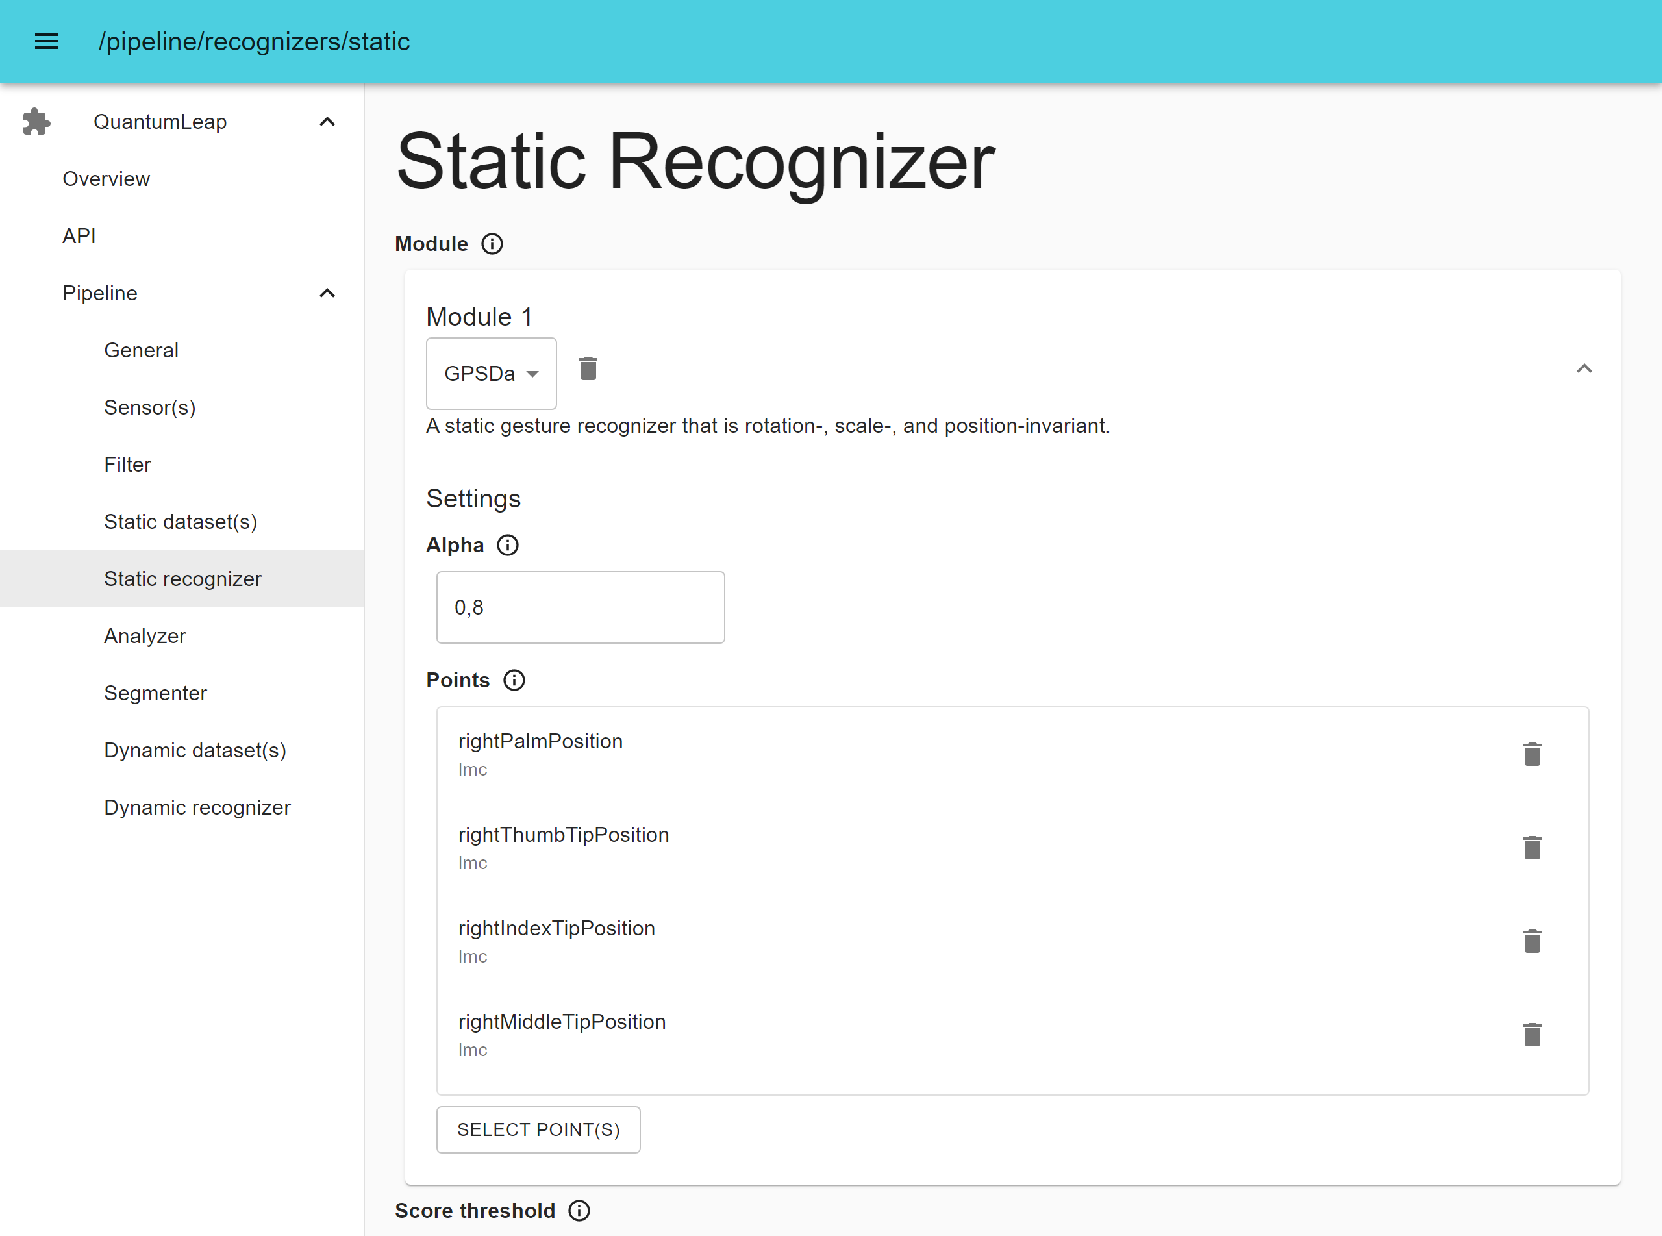
\includegraphics[width=\linewidth]{Figures/QuantumLeap/UI/module-static_recognizer.pdf}  
        \vspace{-15pt}
        \captionsetup{width=.9\linewidth}
        \caption{Static recognizer settings.}
        \label{fig:quantumleap:ui:3}
    \end{subfigure}
    
    \vspace{2pt}
    \begin{subfigure}{.49\textwidth}
        \centering
        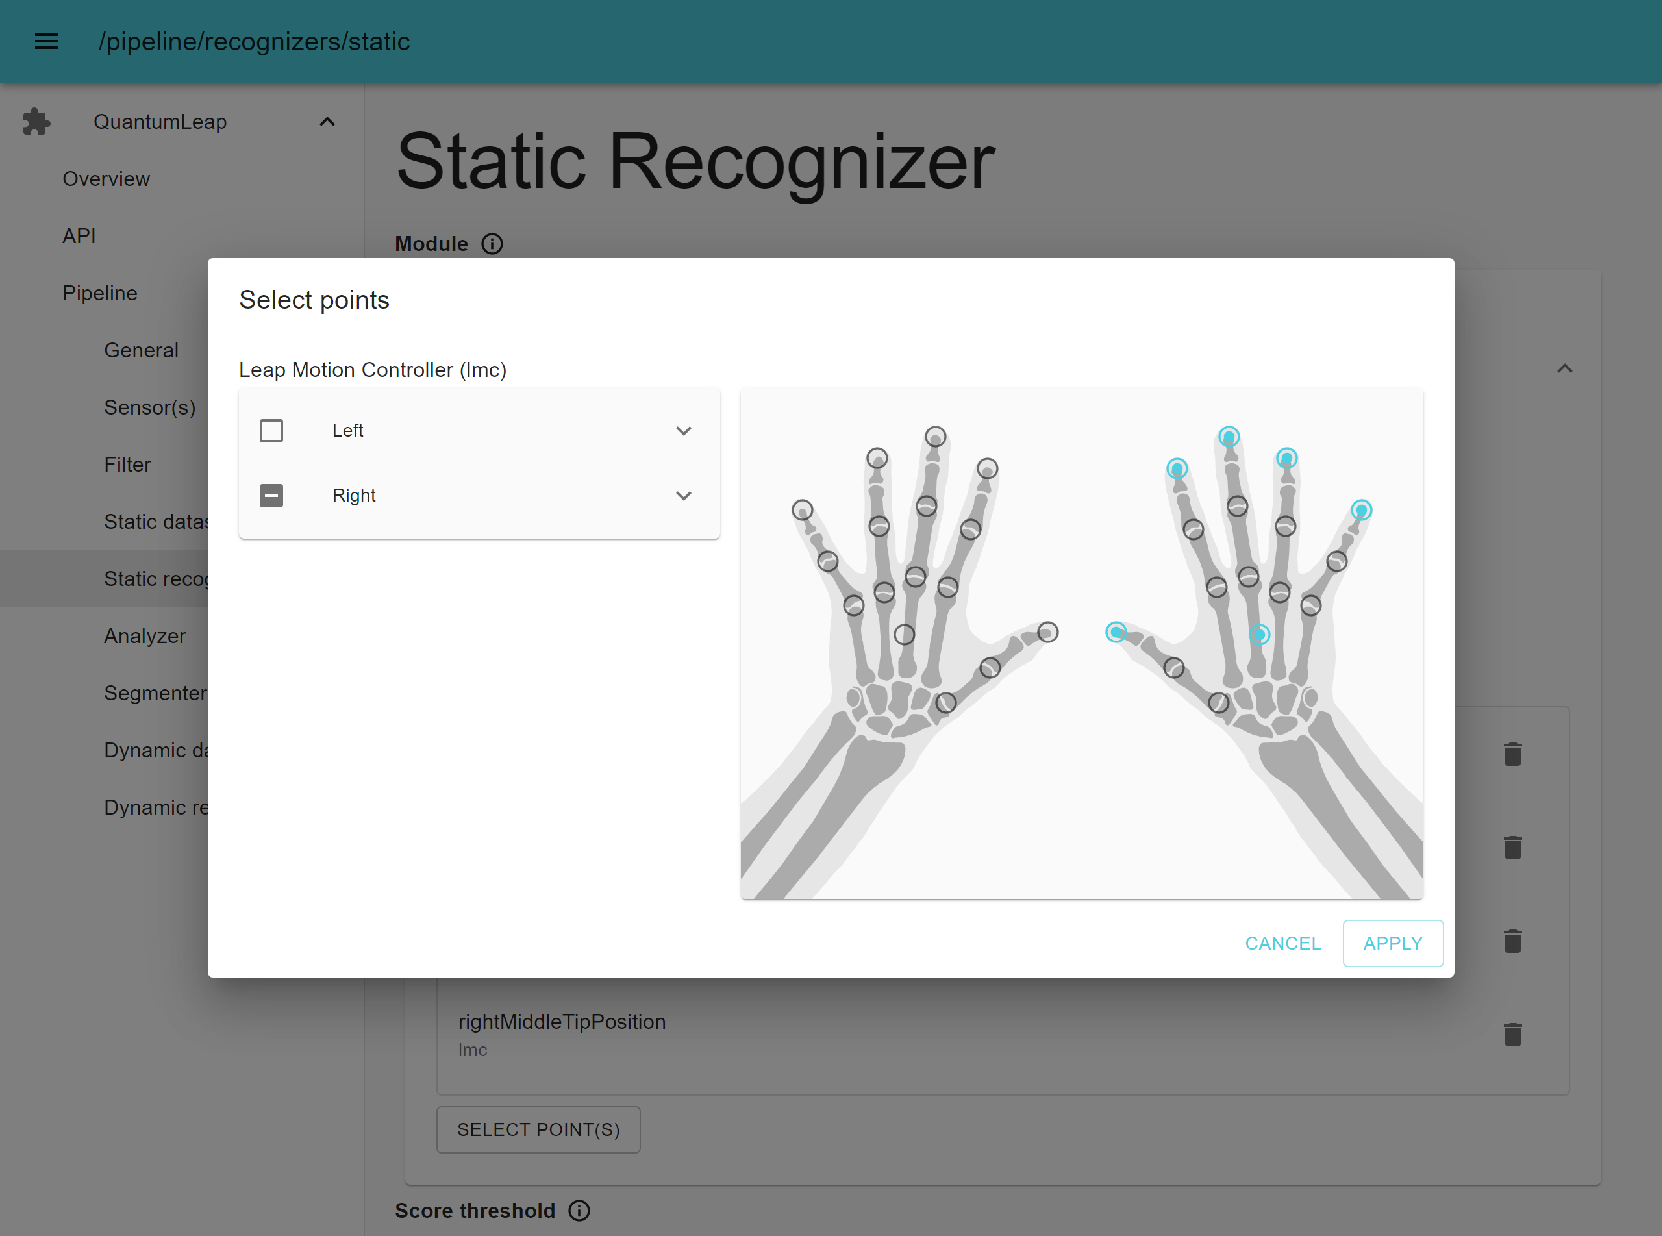
\includegraphics[width=\linewidth]{Figures/QuantumLeap/UI/module-point_selection.pdf}  
        \vspace{-15pt}
        \captionsetup{width=.9\linewidth}
        \caption{Point selection.}
        \label{fig:quantumleap:ui:4}
    \end{subfigure}
    \begin{subfigure}{.49\textwidth}
        \centering
        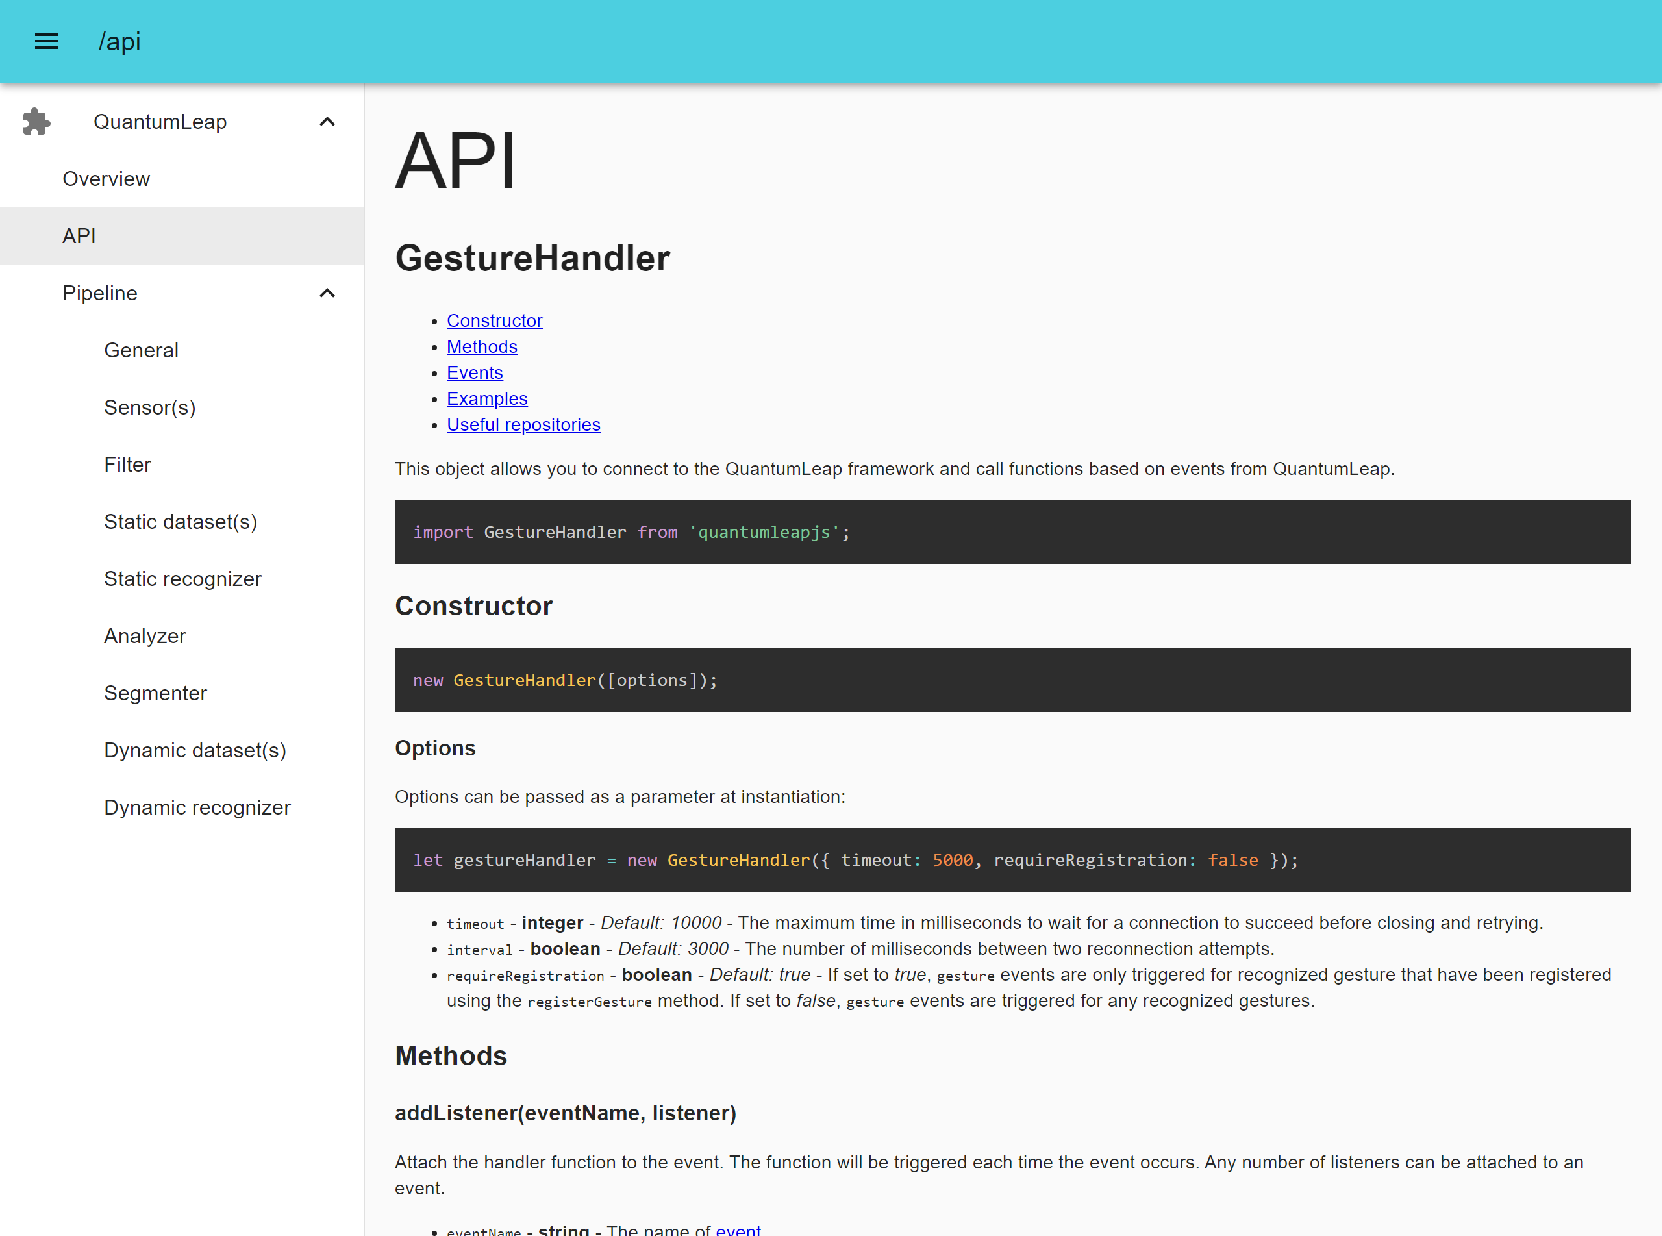
\includegraphics[width=\linewidth]{Figures/QuantumLeap/UI/api.pdf}  
        \vspace{-15pt}
        \captionsetup{width=.9\linewidth}
        \caption{API documentation.}
        \label{fig:quantumleap:ui:2}
    \end{subfigure}

    % \vspace{-4pt}
    \caption{Screenshots of the \ql GUI.}
    \label{fig:quantumleap:ui}
    % \vspace{-12pt}
\end{figure}

\ql features a configuration graphical user interface (GUI) that allows developers to quickly set it up for their needs. It is divided into a series of pages: an ``overview'' page which shows the complete dataflow architecture and allows users to navigate to the page of each module (\fig~\ref{fig:quantumleap:ui:1}), an ``API'' page that contains the complete API documentation (\fig~\ref{fig:quantumleap:ui:2}), and dedicated ``module'' pages for each type of module (\fig~\ref{fig:quantumleap:ui:3} and \ref{fig:quantumleap:ui:4}). The ``module'' pages let developers select a specific implementation of the module and configure it to their needs (\eg select the points used by a recognizer). The settings of each module can be defined in their corresponding ``config-template.json'' file. Framework configurations can be imported and exported as JSON files from the GUI.

The GUI provides limited guidance in the form of short descriptions for each implemented module to help developers select the best set of modules for their application. Further guidance, such as recommending the most appropriate modules (\eg gesture recognizers) for a particular application, is currently outside of the scope of this paper. 
However, resources like the comparative studies of Magrofuoco \etal~\cite{Magrofuoco:2021} or Erazo and P\'erez-Medina~\cite{Erazo:2020} may prove extremely valuable when choosing, \eg a gesture recognizer. 



%--------------------------------------------------------------------------------%
\subsection{Application Programming Interface} \label{sec:quantumleap:description:api}

The \ql API exposes the \custominlinecode{GestureHandler} class, a member of the \custominlinecode{EventEmitter} class of the Node.js core API. A \custominlinecode{GestureHandler} object attempts to connect to a running instance of the \ql framework. It then emits events based on the data received from \ql. %(\eg ``frame'' events are emitted for each frame received and ``gesture'' events are emitted for each recognized gesture). 
The reliance on a standard event-driven architecture should flatten the learning curve for front-end developers and facilitate the transition to gestural UIs, as events are already an integral part of modern UIs. The methods provided by the \custominlinecode{GestureHandler} class include:
\begin{itemize}[noitemsep]
    \item \custominlinecode{connect([address])}: connect to a running instance of \ql.
    \item \custominlinecode{disconnect()}: disconnect from \ql.
    \item \custominlinecode{registerGestures(type, names)}: register gestures to \ql, to enable their recognition.
    \item \custominlinecode{unregisterGestures(type, names)}: unregister gestures to stop them from being recognized.
    \item \custominlinecode{addListener(eventName, listener)}: attach a listener to a particular event. Possible events include:
    \begin{itemize}[noitemsep]
        \item \custominlinecode{frame}: a frame has been received from \ql.
        \item \custominlinecode{gesture}: a gesture (static or dynamic) has been recognized.
        \item \custominlinecode{connect}: the application has connected to \ql.
        \item \custominlinecode{disconnect}: the application has disconnected from \ql.
    \end{itemize}
    \item \custominlinecode{removeListener(eventName, listener)}: remove a listener attached to an event.
\end{itemize}

%================================================================================%
\section{Evaluation} \label{sec:quantumleap:evaluation}

The ISO 9241-Part 11~\cite{iso9241} defines the ``Usability'' quality factor appearing in the ISO 25010~\cite{iso25010} as ``\textit{the effectiveness, the efficiency,  and the satisfaction with which specified users achieve specified goals in particular environments}''. Therefore, to evaluate the overall usability of \ql, an experiment was conducted to quantitatively evaluate the task completion rate (to cover effectiveness), the task completion time, and the cognitive workload based on NASA-TLX~\cite{Hart:1988} (to cover efficiency), and the System Usability Scale (SUS)~\cite{Brooke:1996} to assess its overall usability (to also cover satisfaction). This section describes the evaluation procedure and discusses its results.

%--------------------------------------------------------------------------------%
\subsection{Experiment Protocol} \label{sec:quantumleap:evaluation:protocol}

\subsubsection{Environment}
Participants were sitting in front of a computer in a quiet room. An LMC was already set up and placed in front of them. Each participant was provided with two elements: 
\begin{itemize}
    \item A small React web application consists of four buttons linked to four gestures (``left swipe'', ``right swipe'', ``thumb'', and ``point index''). Clicking on a button displays the type, name, and image representation of the gesture on the screen.
    \item The \ql framework, including the documentation of its API. The configuration of the framework was reset before each experiment.
\end{itemize}

% \subsubsection{Consent}
% Before the experiment, participants were introduced to the procedure and informed that they could leave the experiment at any time. They were then invited to sign a GDPR-compliant consent form and fill in a demographic survey with their age, highest education level, current occupation, estimated number of years of experience in the field of computer science, and estimated expertise in development based on the nine expertise levels defined by Costabile \etal~\cite{Costabile:2008} (\fig~\ref{fig:quantumleap:expertise}).

\subsubsection{Participants}
A purposive and snowball sampling was used to recruit 7 participants (all males), aged between 21 and 27 years old ($M{=}23.3$, $SD{=}1.9$), who volunteered for the experiment. They reported between 1 and 7 years of experience in the field of computer science ($M{=}4.9$, $SD{=}2.2$), and expertise levels ranging from 5 to 9 ($M{=}7.6$, $SD{=}1.8$). Education levels included bachelor's degree (4 participants) and master's degree (3 participants). Our criteria for inclusion in this experiment required participants to have at least one year of professional development experience.

\subsubsection{Procedure and Tasks}
The experiment consisted of one session taking around 80 minutes per participant. A session consisted of six phases:

\begin{figure}[tb]
    \centering
    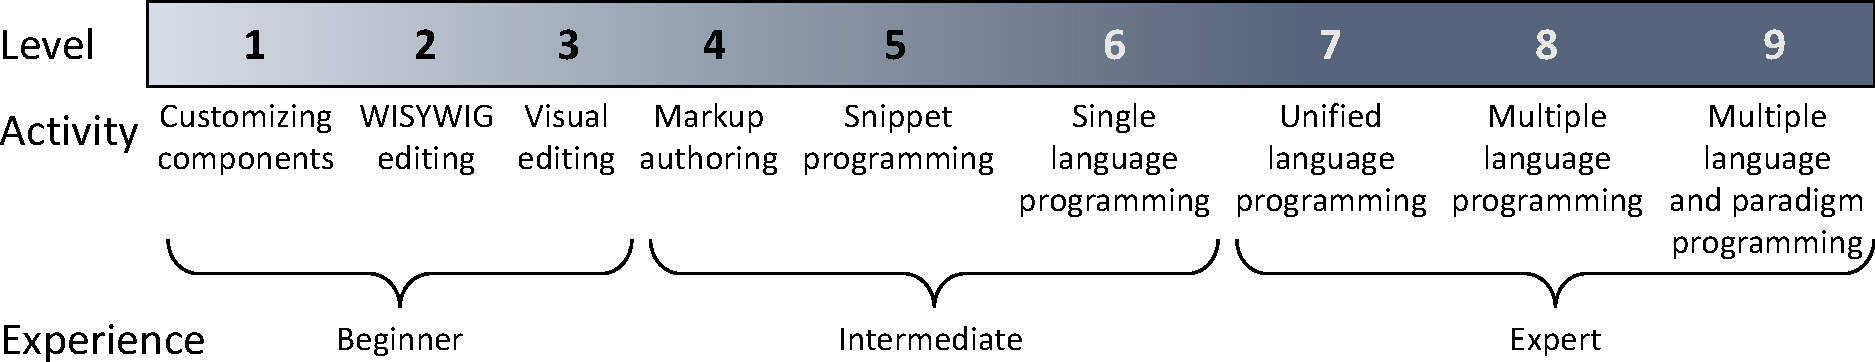
\includegraphics[width=\linewidth]{Figures/QuantumLeap/Evaluation/expertise-levels.pdf}
    \vspace{-8pt}
    \caption{The nine development expertise levels~\cite{Costabile:2008}.} %,Vanderdonckt:2019a}.}
    % \vspace{-8pt}
    \label{fig:quantumleap:expertise}
\end{figure}

\begin{enumerate}
    \item \textit{Consent form and demographic information.} Participants were introduced to the procedure and informed that they could leave the experiment at any time. They were then invited to sign a GDPR-compliant consent form and fill in a demographic survey with their age, highest education level, current occupation, estimated number of years of experience in the field of computer science, and estimated expertise in development based on the nine expertise levels defined by Costabile \etal~\cite{Costabile:2008} (\fig~\ref{fig:quantumleap:expertise}).
    \item \textit{Introduction phase.} Participants were introduced to the application and the \ql framework. They were given a few minutes to try them out and analyze the source code of the application before continuing the experiment.
    \item \textit{Configuration phase.} Participants configured the \ql framework for the application with its configuration GUI. This task comprised seven steps, detailed in Appendix~\ref{app:quantumleap-tasks:tasks-config}.
    \item \textit{Development phase.} Participants modified the source code of the application to make it react to static and dynamic hand gestures. This task comprised 13 steps, detailed in Appendix~\ref{app:quantumleap-tasks:tasks-dev}.
    \item \textit{Questionnaires.} Participants were asked to complete two questionnaires: the System Usability Scale (SUS) questionnaire~\cite{Brooke:1996} and the NASA-Task Load Index (NASA-TLX) questionnaire~\cite{Hart:1988}. 
    %
    SUS comprises ten questions evaluating the usability of a system (in this case, \ql) and has been selected for its proven reliability~\cite{Bangor:2008} and efficient administration. 
    %
    NASA-TLX assesses the estimated workload of the \textit{configuration} and \textit{development} tasks and comprises six subscales: mental demand, physical demand, temporal demand, effort, performance, and frustration level. Each subscale is assigned a weight determined by asking the participant to select the subscale that contributes the most to the workload in 15 pairwise comparisons. In this way, each participant was able to express which subscale is perceived as the most important with respect to others, as opposed to maintaining the same weight for all subscales. Pandian and Tuleri's NASA-TLX software~\cite{Pandian:2020} was used to simplify the process of data collection and analysis (\fig~\ref{fig:quantumleap:nasa-tlx-app}).
    \item \textit{Open-ended questions and comments.} Participants answered four questions to provide insights on their overall feelings:
    \begin{itemize}[noitemsep]
        \item If you did not complete all the tasks, what was the reason?
        \item What did you think of \ql?
        \item What did you like?
        \item What would you change?
    \end{itemize}
\end{enumerate}


% Participants were first introduced to the application and the \ql framework. They were given a few minutes to try them out and look at the source code of the application before continuing the experiment. The rest was divided into five tasks:
% \begin{enumerate}[noitemsep]
%     \item \textit{Configuration}: the participants configure the \ql framework for the application with its configuration UI. This task comprises 7 steps, detailed in Appendix~\ref{app:quantumleap-tasks:tasks-config}.
%     \item \textit{Development}: the participants modify the source code of the application to make it react to static and dynamic hand gestures. This task comprises 13 steps, detailed in Appendix~\ref{app:quantumleap-tasks:tasks-dev}.
%     \item \textit{SUS Questionnaire}: once the participants had finished the above two tasks and their related steps, they were asked to fill out the System Usability Scale (SUS) questionnaire~\cite{Brooke:1996}, which comprises ten questions evaluating the usability of a system (in this case, \ql). This questionnaire has been selected for its proven reliability~\cite{Bangor:2008} and its efficient administration.
%     \item \textit{NASA-TLX Questionnaire}: participants were then asked to fill out the NASA-Task Load Index (NASA-TLX) questionnaire~\cite{Hart:1988}, which assesses the estimated workload of the \textit{configuration} and \textit{development} tasks. It consists of six subscales: mental demand, physical demand, temporal demand, effort, performance, and frustration level. Each subscale is then assigned a weight that is determined by asking the participant to select the subscale that contributes the most to the workload in 15 pairwise comparisons. In this way, each participant was able to express which subscale is perceived as the most important with respect to others, as opposed to maintaining the same weight for all subscales. Pandian and Tuleri's NASA-TLX software~\cite{Pandian:2020} was used to simplify the process of data collection and analysis (\fig~\ref{fig:quantumleap:nasa-tlx-app}).
%     \item \textit{Open-Ended Questions and Comments}: the participants answer the following four open-ended questions to provide insights on their overall feelings:
%     \begin{itemize}[noitemsep]
%         \item If you did not complete all the tasks, what was the reason?
%         \item What did you think of \ql?
%         \item What did you like?
%         \item What would you change?
%     \end{itemize}
% \end{enumerate}

% Each evaluation took approximately ~80 minutes per participant.

\begin{figure}[h]
    \centering
    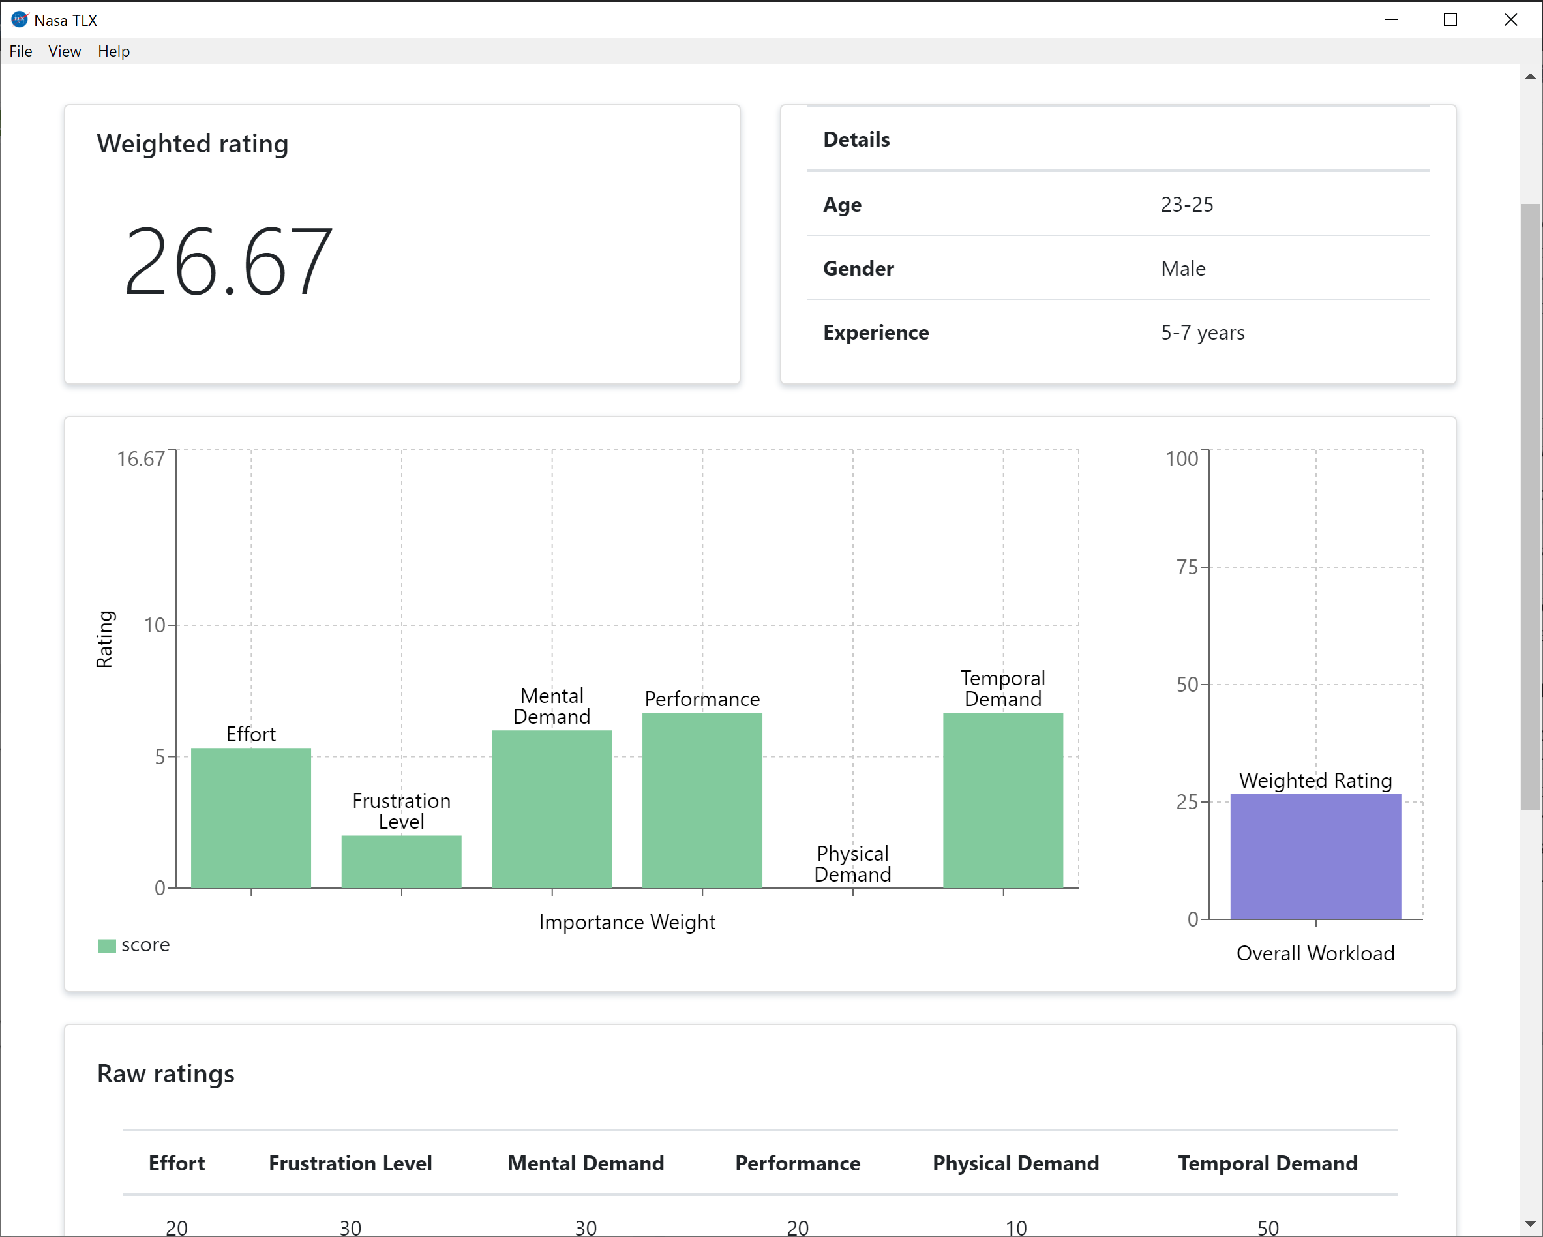
\includegraphics[width=\linewidth]{Figures/QuantumLeap/Evaluation/NASA-TLX.pdf}
    % \vspace{-8pt}
    \caption{NASA-TLX software~\cite{Pandian:2020} screenshot showing results of a participant: the overall weighted rating, the rating per subscale, and the individual weights for each subscale.}
    \label{fig:quantumleap:nasa-tlx-app}
    % \vspace{-8pt}
\end{figure}

\subsubsection{Metrics and Data Collection}
We collected a set of metrics for the configuration and development phases of the experiment to provide insight into the efficiency and effectiveness of \ql:
\begin{enumerate}
    \item The \textsc{Task success rate} is the ratio between the number of steps completed successfully by a participant and the total number of steps required to complete the procedure.
    \item The \textsc{Task completion time} measures the time taken by the participant for each of the configuration and development tasks.
    \item The \textsc{Step completion time} measures the time taken to perform each step of each of the two aforementioned tasks.
\end{enumerate}
In addition to these metrics, we collected demographic information, as well as answers to the SUS questionnaire, NASA-TLX questionnaire, and open-ended questions.

%--------------------------------------------------------------------------------%
\subsection{Results and Discussion} \label{sec:quantumleap:evaluation:results}

\subsubsection{Task Success Rate}
Despite their differences in terms of years of experience and level of expertise, six of the seven participants ($\frac{6}{7}{=}86\%$) completed all the steps of each task without any issue on the first run. Only one participant initially performed the fifth step of the \textit{Development} task incorrectly. However, this participant immediately realized his mistake and subsequently corrected it after completing the next step, ultimately resulting in a task success rate of 100\%. This suggests that the effectiveness is well covered by \ql.

\subsubsection{Task and Step Completion Times}
As a potential optimal performance, the first author of this paper (23 years, 6 years of experience, level 8)  completed the \textit{Configuration} and \textit{Development} tasks of the experiment in 2.1 minutes and 10.2 minutes, respectively. On average, participants took 6.6 minutes to complete the first task ($SD{=}1.2$), with the slowest participant completing it in 9.1 minutes and the fastest in 5.2 minutes. For the second task, the completion time was between 22.2 and 65.1 minutes ($M{=}37.4$, $SD{=}18.2$). \fig~\ref{fig:quantumleap:task2-time} shows that participants spent a more significant amount of time on the fifth step of this task (\ie adding an event listener that reacts to the ``swipe left'' gesture), which is normal since this is the most complex step.

\begin{figure}[t]
    \centering
    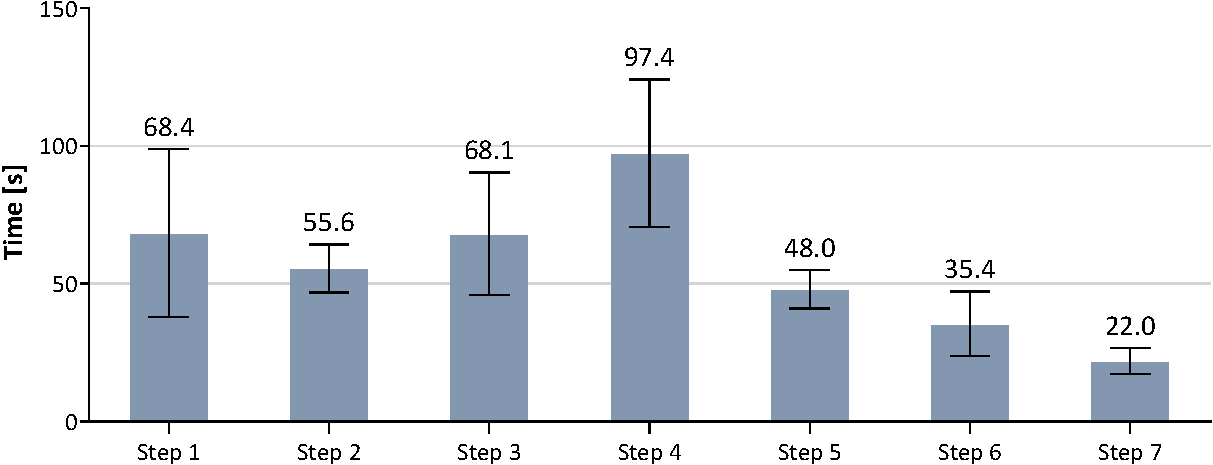
\includegraphics[width=\linewidth]{Figures/QuantumLeap/Evaluation/Task 1 (time).pdf}
    % \vspace{-14pt}
    \caption{Average time for each step of the \textit{Configuration} task. Error bars show a confidence interval with $\alpha{=}0.5$.}
    \label{fig:quantumleap:task1-time}
    % \vspace{-8pt}
\end{figure}


While steps five and eight are similar, participants took seven times longer to perform the former than the latter. A plausible explanation could be that the first time they encountered the problem of reacting to a gesture, participants took some time to check the API before modifying the source code of the application. When they mastered the API, participants could then quickly complete the remaining steps.


\begin{figure}[t]
    \centering
    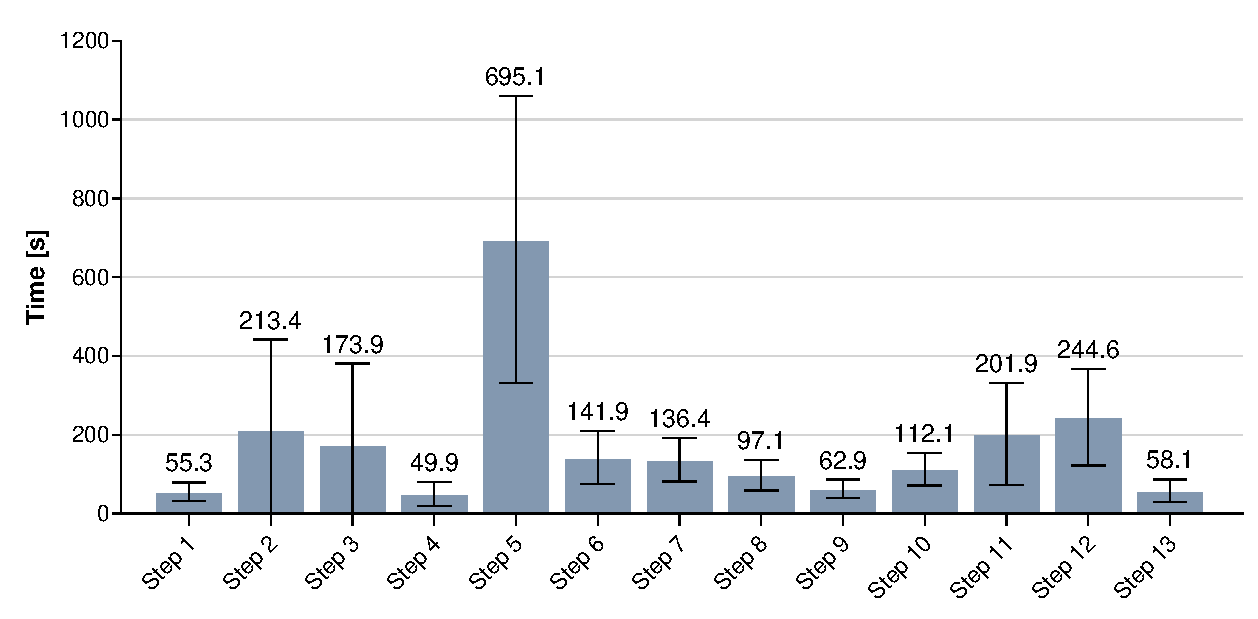
\includegraphics[width=\linewidth]{Figures/QuantumLeap/Evaluation/Task 2 (time).pdf}
    % \vspace{-18pt}
    \caption{Average time for each step of the \textit{Development} task. Error bars show a confidence interval with $\alpha{=}0.5$. Note that one participant performed tasks 8, 9, and 10 in parallel. The participant's time for each of these tasks was thus inferred from the total time to perform the three tasks and the ratio between the average time for these tasks.}
    \label{fig:quantumleap:task2-time}
\end{figure}

To investigate the relationship between participants' expertise and their task completion time, we compute a Spearman's rank correlation between participants' reported level of expertise in development and their completion time for the \textit{Configuration} and \textit{Development} tasks. While no significant correlation was observed between the completion time of the first task and the expertise level, thus suggesting that the configuration GUI is perceived with a similar easiness regardless of the skill level, the completion time of the second task significantly correlates with expertise ($r{=}-.93$, $p{=}.002^{**}$). This result was expected, as the second task of the experiment requires participants to leverage their programming skills to modify the source code of the application. 

\subsubsection{SUS Questionnaire}
Since the answers to the SUS questionnaire were not normally distributed based on a Shapiro-Wilk test (\eg for question 3, $W{=}0.45$, $p{<}.001^{***}$), we investigated the overall appreciation of the participants by conducting a one-sample Wilcoxon test comparing their answers to the midpoint of the scale (\ie 3.0). For odd-numbered, resp. for even-numbered questions, an answer is considered positive if it is significantly higher, resp. lower than the midpoint value. All odd-numbered, resp. even-numbered, questions received a mean higher, resp. lower than the midpoint of the scale, thus representing an already positive assessment. Furthermore, six of the ten questions are statistically significantly different from the midpoint value, suggesting an even more positive answer for these questions: question 1 ($W{=}21.0$, $p{=}.031^*$), question 3 ($W{=}28.0$, $p{=}.016^*$), question 5 ($W{=}21.0$, $p{=}.031^*$), question 6 ($W{=}{-}21.0$, $p{=}.031^*$), question 7 ($W{=}28.0$, $p{=}.016^*$), and question 10 ($W{=}{-}21.0$, $p{=}.031^*$).
As recommended by Brooke~\cite{Brooke:1996} and Bangor \etal~\cite{Bangor:2008}, we also analyzed the SUS questionnaire as a whole. SUS scores range between 62.5 and 85.0 out of 100 ($M{=}77.9$, $SD{=}7.8$), resulting in a rating of B+ (``good'') on Sauro's rating scale~\cite{Sauro:2010}, which denotes a reasonable level of usability for such an environment. According to Lewis and Sauro~\cite{Lewis:2009}, the overall SUS score can be further divided into two subcomponents, namely learnability and usability. Learnability is computed by summing the scores of questions 4 and 10 of the questionnaire and multiplying the result by 12.5. Usability is computed by summing the scores of the other questions and multiplying the result by 3.125. QuantumLeap obtains a mean learnability score of 78.6 and a usability score of 77.7. 

To investigate the internal consistency reliability among participants, we also computed Guttman's $\lambda_4{=}.91$ coefficient~\cite{Guttman:1945} with $n{=}2,000$ iterations. This value is above $\lambda_4{\geq}.90$ which represents the highest rank of consistency, usually required for high-stakes decisions like school admissions~\cite{Callender:1979}, thus suggesting that participants consistently answered the SUS questionnaire and that their answers were reliable enough.
Guttman’s $\lambda_4$ coefficient represents a good measure of reliability that produces a  value higher than the usual Cronbach’s $\alpha$, but with a positive bias likely to be small if the estimated reliability is larger than 0.85 (which is the case here) when the sample is small ($n{=}7$). After computing the Spearman's rank correlation between participants' SUS scores and their reported level of expertise, we observe a positive correlation ($r{=}.82$, $p{=}.033^*$), which suggests that the system feels more usable to experienced users than to intermediary ones.

\subsubsection{NASA-TLX Questionnaire}
% Graph with weighted scores
Workload scores range from 8.7 to 65.3 out of 100 ($M{=}34.0$, $SD{=}19.5$). According to Grier~\cite{Grier:2015}, who analyzed the NASA-TLX scores of 37 computer activities, the measured workload for \ql falls into the second quartile (score lower than 54.0). Each participant managed to complete all steps of the experiment and some even reported being impressed by the results, considering that they would not have been able to do the same without the help of the framework. This could explain the low impact of the ``performance subfactor''. 
 Contrarily to the SUS score, no significant correlation was observed between participants' workload scores and their reported level of expertise after computing Spearman's rank correlation.

\begin{figure}[t]
    \centering
    \vspace{4pt}
    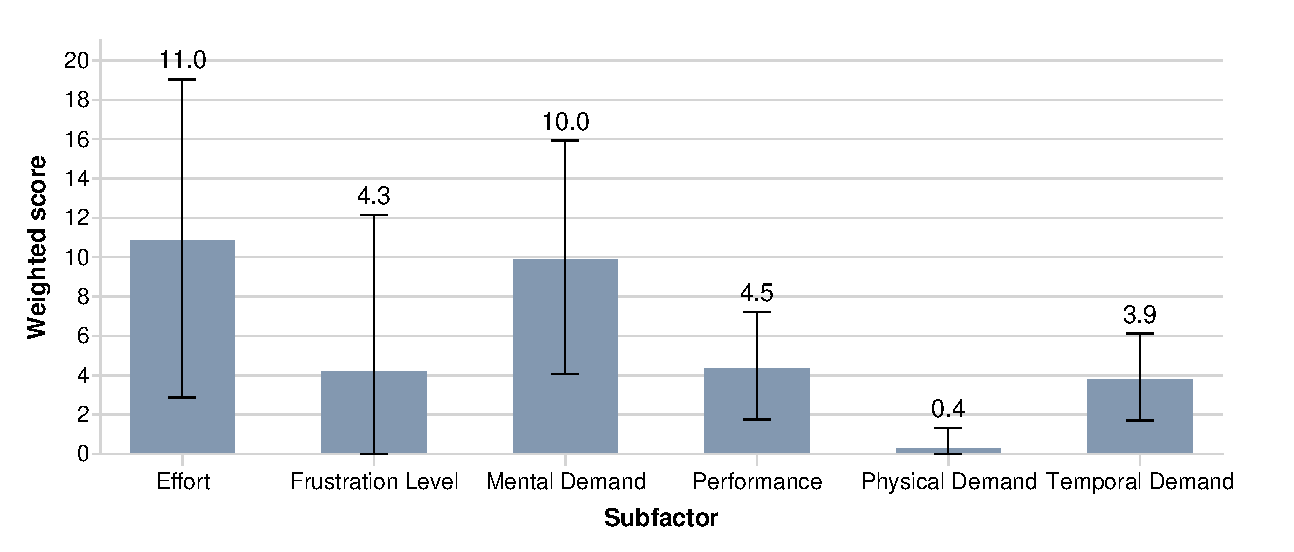
\includegraphics[width=\linewidth]{Figures/QuantumLeap/Evaluation/NASA-TLX-scores.pdf}
    \caption{Average weighted score for each subscale of the NASA-TLX questionnaire. Error bars show a confidence interval with $\alpha{=}0.5$.}
    % \vspace{-8pt}
    \label{fig:quantumleap:nasa-tlx-scores}
\end{figure}

\begin{table}[t]
    \footnotesize
    \centering
    \begin{tabular}{lrr}
        \toprule
        \multirow{2}{*}{\textbf{Subscale}} & \multicolumn{2}{c}{\textbf{Score}} \\
         & M & SD \\
        \midrule
        Mental Demand & 10.0 & 6.4 \\
        Physical Demand & 0.4 & 1.0 \\
        Temporal Demand & 3.9 & 2.4 \\
        Effort & 11.0 & 8.7 \\
        Performance & 4.5 & 2.9 \\
        Frustration level & 4.3 & 8.5 \\
        \midrule
        Overall & 34.0 & 19.5 \\
        \bottomrule
    \end{tabular}
    \caption{Average weighted score and standard deviation for each subscale of the NASA-TLX questionnaire.}
    % \vspace{-18pt}
    \label{tbl:quantumleap:nasa-tlx}
\end{table}

\subsubsection{Open-Ended Questions}
Overall, participants found that adding gesture support to an application was surprisingly quick and easy. However, some participants expressed some concern about not being able to configure the dataflow correctly without external help. Their remarks and suggestions are summarized as follows:
\begin{enumerate}[noitemsep]
    \item \textit{Configuration}. Comments targeting the configuration process, the GUI, and the usability.
    \begin{itemize}[noitemsep]
        \item There should be some feedback to indicate to the user that the framework is starting/stopping ($\frac{6}{7}{=}86\%$). 
        \item There should be some feedback to notify the user that the settings were successfully saved ($\frac{5}{7}{=}71\%$).
        \item After selecting a module, its settings should be displayed by default, instead of having to click to display them ($\frac{5}{7}{=}71\%$).
        \item A lot of steps are required to configure the dataflow ($\frac{2}{7}{=}29\%$).
        \item There should be a button to add a module, instead of just selecting the module in a drop-down menu ($\frac{2}{7}{=}29\%$).
        \item There should be a tutorial that provides guidance on dataflow configuration ($\frac{1}{7}{=}14\%$).
        \item There are some inconsistencies in the GUI ($\frac{1}{7}{=}14\%$).
        \item There should be a simple way to switch from right-handed gestures to left-handed ($\frac{1}{7}{=}14\%$).
    \end{itemize}
    \item \textit{Development}. Comments targeting the development of a gesture-based application using the \ql API.
    \begin{itemize}[noitemsep]
        \item There should be a method to directly attach a listener to a specific gesture, instead of having to listen to the generic ``gesture'' event and then check the gesture name ($\frac{2}{7}{=}29\%$).
        \item The API documentation should provide the data types of event properties ($\frac{1}{7}{=}14\%$).
        \item The API documentation should clearly show the link between listeners and events ($\frac{1}{7}{=}14\%$).
        \item The distinction between static and dynamic gestures may be confusing ($\frac{1}{7}{=}14\%$).
    \end{itemize}
    \item \textit{Experiment} Comments targeting the experiment itself (\eg unclear steps).
    \begin{itemize}[noitemsep]
        \item The order of some steps was confusing. In particular, the call to \custominlinecode{registerGesture} should have been introduced before the call to \custominlinecode{addListener} ($\frac{2}{7}{=}29\%$). 
        \item In step three of the second task, the address and port of the running instance of \ql should have been provided ($\frac{2}{7}{=}29\%$). 
    \end{itemize}
\end{enumerate}

\subsubsection{Limitations of the Study}
This study is subject to two main limitations, which could influence the validity of its outcomes.
%
First, the substantial guidance provided during the ``configuration'' phase of the study poses a threat to its external validity~\cite{Feldt:2010}, as our findings may not generalize to a real-life scenario in which no such guidance is available. 
%
Second, the study would have benefited from incorporating an A/B comparison between the development of a gesture-based application with and without \ql to better highlight its impact in terms of time, effort, and the overall quality of the resulting work.

%--------------------------------------------------------------------------------%
\subsection{Changes} \label{sec:quantumleap:evaluation:changes}
Following this experiment, we are planning on improving \ql based on the aforementioned participants' comments.

\subsubsection{Short-term Changes} The most requested changes have already been implemented in the latest version of \ql. They include:
\begin{itemize}
    \item Displaying a loading icon in the GUI when \ql is starting\slash stopping.
    \item Displaying a message in the GUI when the settings have been saved.
    \item Displaying the settings of modules by default in the GUI, instead of requiring the user to click on a button to display them.
\end{itemize}

\subsubsection{Long-term Changes} 
We believe that these long-term changes would prove especially useful for less experienced developers:
\begin{itemize}
    \item Add the possibility to attach listeners to specific gestures in one step, instead of requiring developers to listen to the generic ``gesture'' event.
    \item Propose a set of default configurations to allow developers to quickly prototype gesture-enabled applications without having to build a complete dataflow configuration.
    \item Create an interactive tutorial that guides users through the configuration of the \ql dataflow.
    \item Automatically configure the dataflow based on the selected gesture set and target usage. For instance, \ql could suggest a segmenter that is well-suited to the environment and determine the most accurate recognizers for the gesture set.
\end{itemize}


%================================================================================%
\section{Sensor Integration and Applications} \label{sec:quantumleap:integration}
Through the years, additional sensors were implemented into \ql by students for use in their master's thesis, showing that \ql can be easily extended with new modules. These sensors and some of their applications are summarized in \tab~\ref{tab:quantumleap:integration}.

In this thesis, we used \ql to build an LMC-based multimedia application called Large User Interface (\lui, \fig~\ref{fig:quantumleap:apps:lui}~\cite{Sluyters:2022:LUI}. This application, its user-centered development method, and its evaluation are described in Chapter~\ref{chap:lui}.
%
With the help of my friends and colleagues Quentin Sellier, Victor Slu\"{y}ters, and Jean-Martin Vlaeminck, we also used \ql during the Citizens of Wallonia hackathon in March 2023 to create Wall'ON (\fig~\ref{fig:quantumleap:apps:wallon}), an interactive kiosk that provides information about works in the city in a fun and intuitive way~\cite{Rawart:2023}.

\begin{table}[!b]
    \renewcommand{\arraystretch}{1.2}
    \footnotesize
    \centering
    \begin{tabular}{l>{\raggedright}p{2.5cm}>{\raggedright}p{1.75cm}ll}
        \toprule    
        \textbf{Sensor(s)} & \textbf{Type} & \textbf{Application Domain} & \textbf{Validation} & \textbf{Reference} \\
        \midrule
        Leap Motion Controller & Vision & Multimedia & S, D, U & This work \\
         &  & Healthcare & S, D & \cite{Nothomb:2020} \\
         &  & Participatory governance & D & \cite{Rawart:2023} \\
        Kinemic & IMUs & Multimedia & S, D & \cite{Steeman:2022} \\
        3D Touchpad & Touch + proximity sensor & N/A & S & \cite{Neuville:2021} \\
        Gheran Ring Device & IMUs & N/A & S & \cite{Lahousse:2022} \\
        Myo Armband & EMG & N/A & S & \cite{Cornet:2023} \\
        Touchscreen & Touch & Smart home & S, D & \cite{Moinnet:2022} \\
        \bottomrule
    \end{tabular}
    \caption{Summary of the sensors included into \ql. Types of validation include system performance (S), demonstration (D), and user study (U).}
    \label{tab:quantumleap:integration}
\end{table}

Nothomb \etal~\cite{Nothomb:2020} introduced a gesture-based DICOM image viewer (\fig~\ref{fig:quantumleap:apps:dicom}) that allowed surgeons to navigate patient images in the operating room more hygienically and efficiently.
%
Chauvaux and Steeman~\cite{Steeman:2022} integrated the Kinemic sensor, an armband that uses Inertial Measurement Units (IMUs) to track arm gestures, into \ql and built a gesture-based presentation application in which users could change slides with simple hand gestures (\fig~\ref{fig:quantumleap:apps:slides}).
%
Gosselin and Moinnet~\cite{Moinnet:2022} used \ql to build a touch-based application that enabled users to record and assign (combinations of) stroke gestures to actions in a smart house, such as turning the lights on (\fig~\ref{fig:quantumleap:apps:smart-home}).

Finally, Neuville~\cite{Neuville:2021}, Lahousse~\cite{Lahousse:2022}, and Cornet~\cite{Cornet:2023} integrated three additional sensors into \ql: (1) the 3D Touchpad, a device that supports touch and 3D gestures performed above its surface, (2) the Phidget ring, which captures 3D hand motion with an accelerometer, and (3) the Myo Armband, an EMG sensor that fits around the arm. They did not develop any application but used \ql to compare various recognizer modules on their gesture set.

\begin{figure}[t]
    \centering
    \begin{subfigure}{.259\textwidth}
        \centering
        \includegraphics[width=\linewidth]{Figures/QuantumLeap/Applications/lui-prototype.pdf}  
        \vspace{-15pt}
        \captionsetup{width=.9\linewidth}
        \caption{LUI.}
        \label{fig:quantumleap:apps:lui}
    \end{subfigure}
    \begin{subfigure}{.337\textwidth}
        \centering
        \includegraphics[width=\linewidth,trim={5cm 0 0 0},clip]{Figures/QuantumLeap/Applications/wallon-prototype.pdf}  
        \vspace{-15pt}
        \captionsetup{width=.9\linewidth}
        \caption{Wall'ON.}
        \label{fig:quantumleap:apps:wallon}
    \end{subfigure}
    \begin{subfigure}{.383\textwidth}
        \centering
        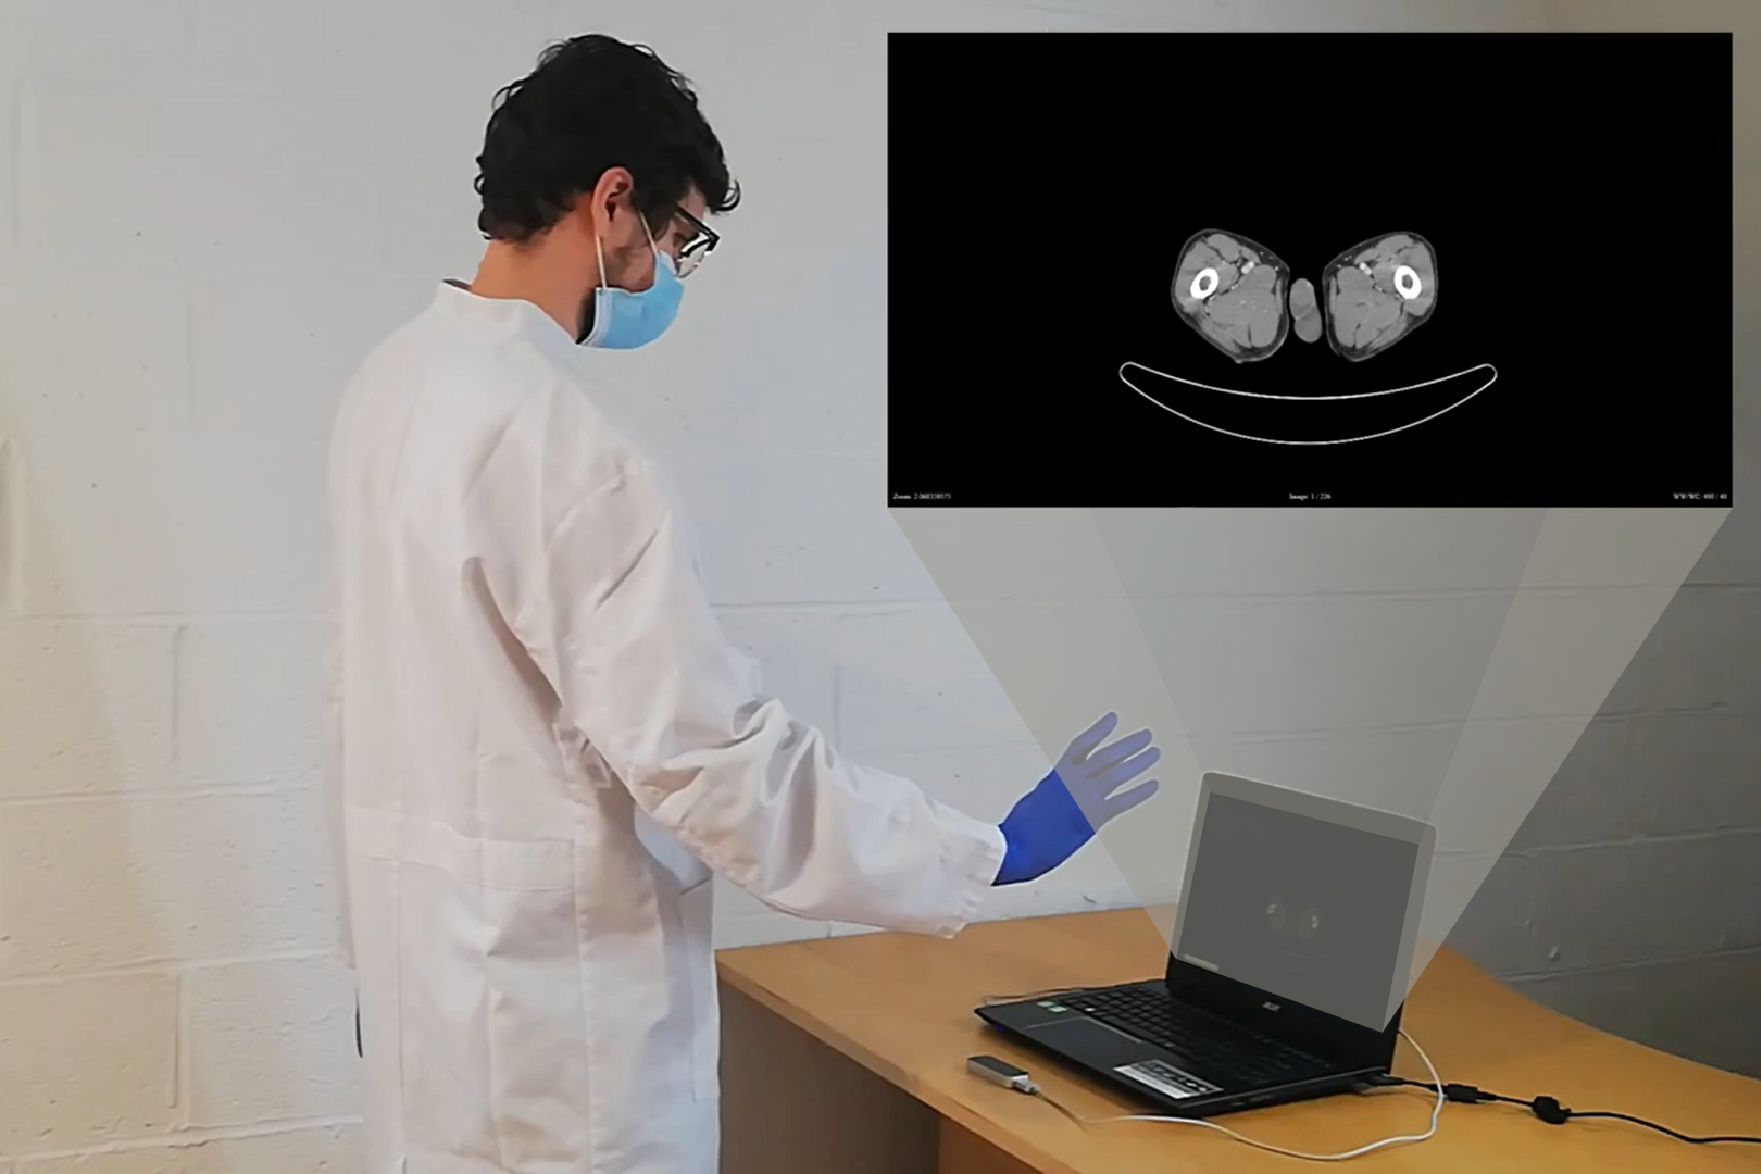
\includegraphics[width=\linewidth,trim={4.5cm 0 0 0},clip]{Figures/QuantumLeap/Applications/dicom-prototype.pdf}  
        \vspace{-15pt}
        \captionsetup{width=.9\linewidth}
        \caption{DICOM viewer~\cite{Nothomb:2020}.}
        \label{fig:quantumleap:apps:dicom}
    \end{subfigure}

    \vspace{2pt}
    \begin{subfigure}{.455\textwidth}
        \centering
        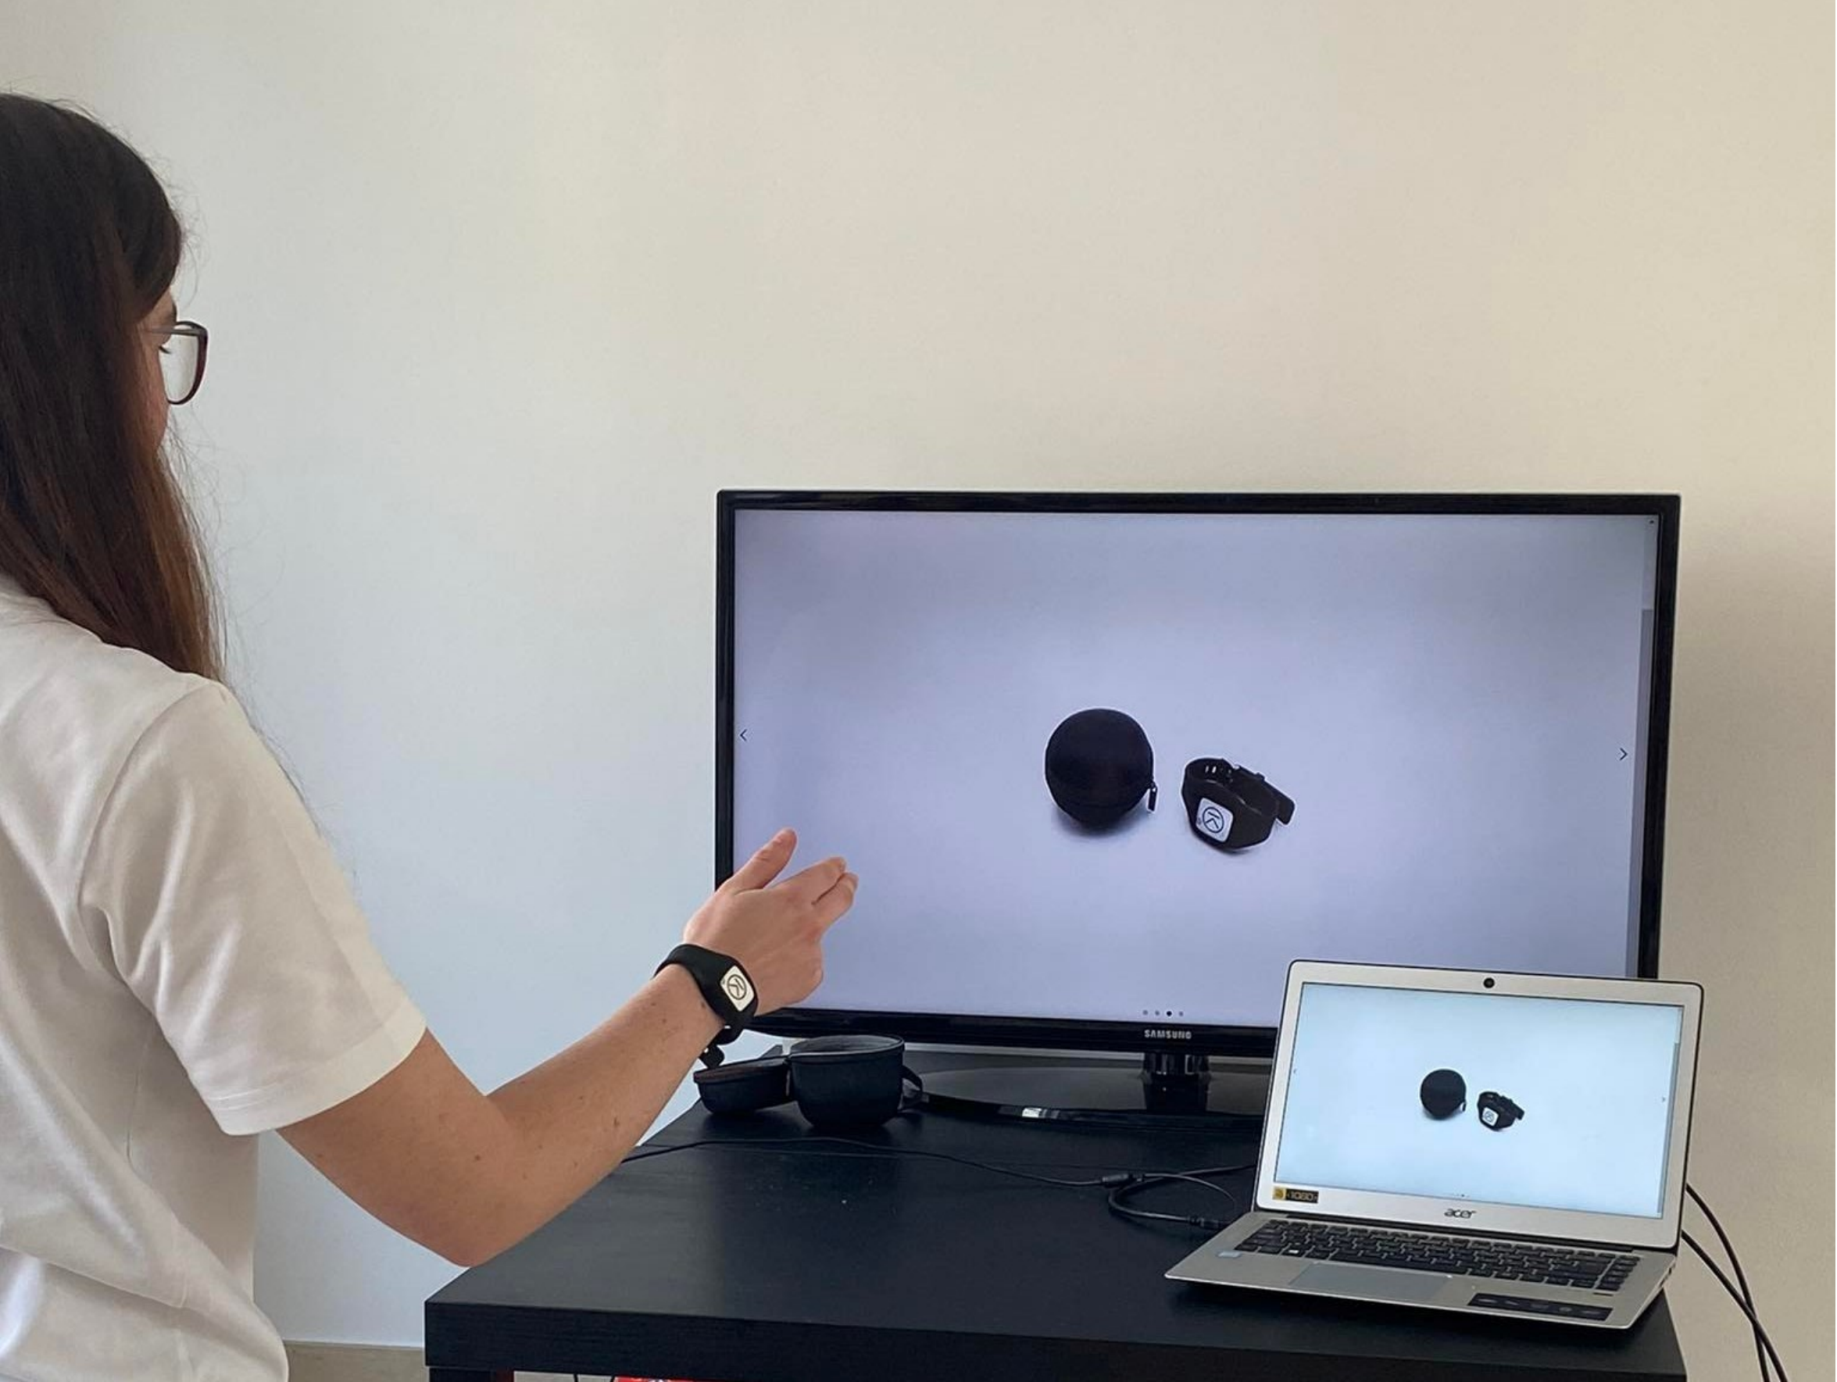
\includegraphics[width=\linewidth,trim={0 0 1cm 0cm},clip]{Figures/QuantumLeap/Applications/slides-prototype.pdf}  
        \vspace{-15pt}
        \captionsetup{width=.9\linewidth}
        \caption{Slides application~\cite{Steeman:2022}.}
        \label{fig:quantumleap:apps:slides}
    \end{subfigure}
    \begin{subfigure}{.535\textwidth}
        \centering
        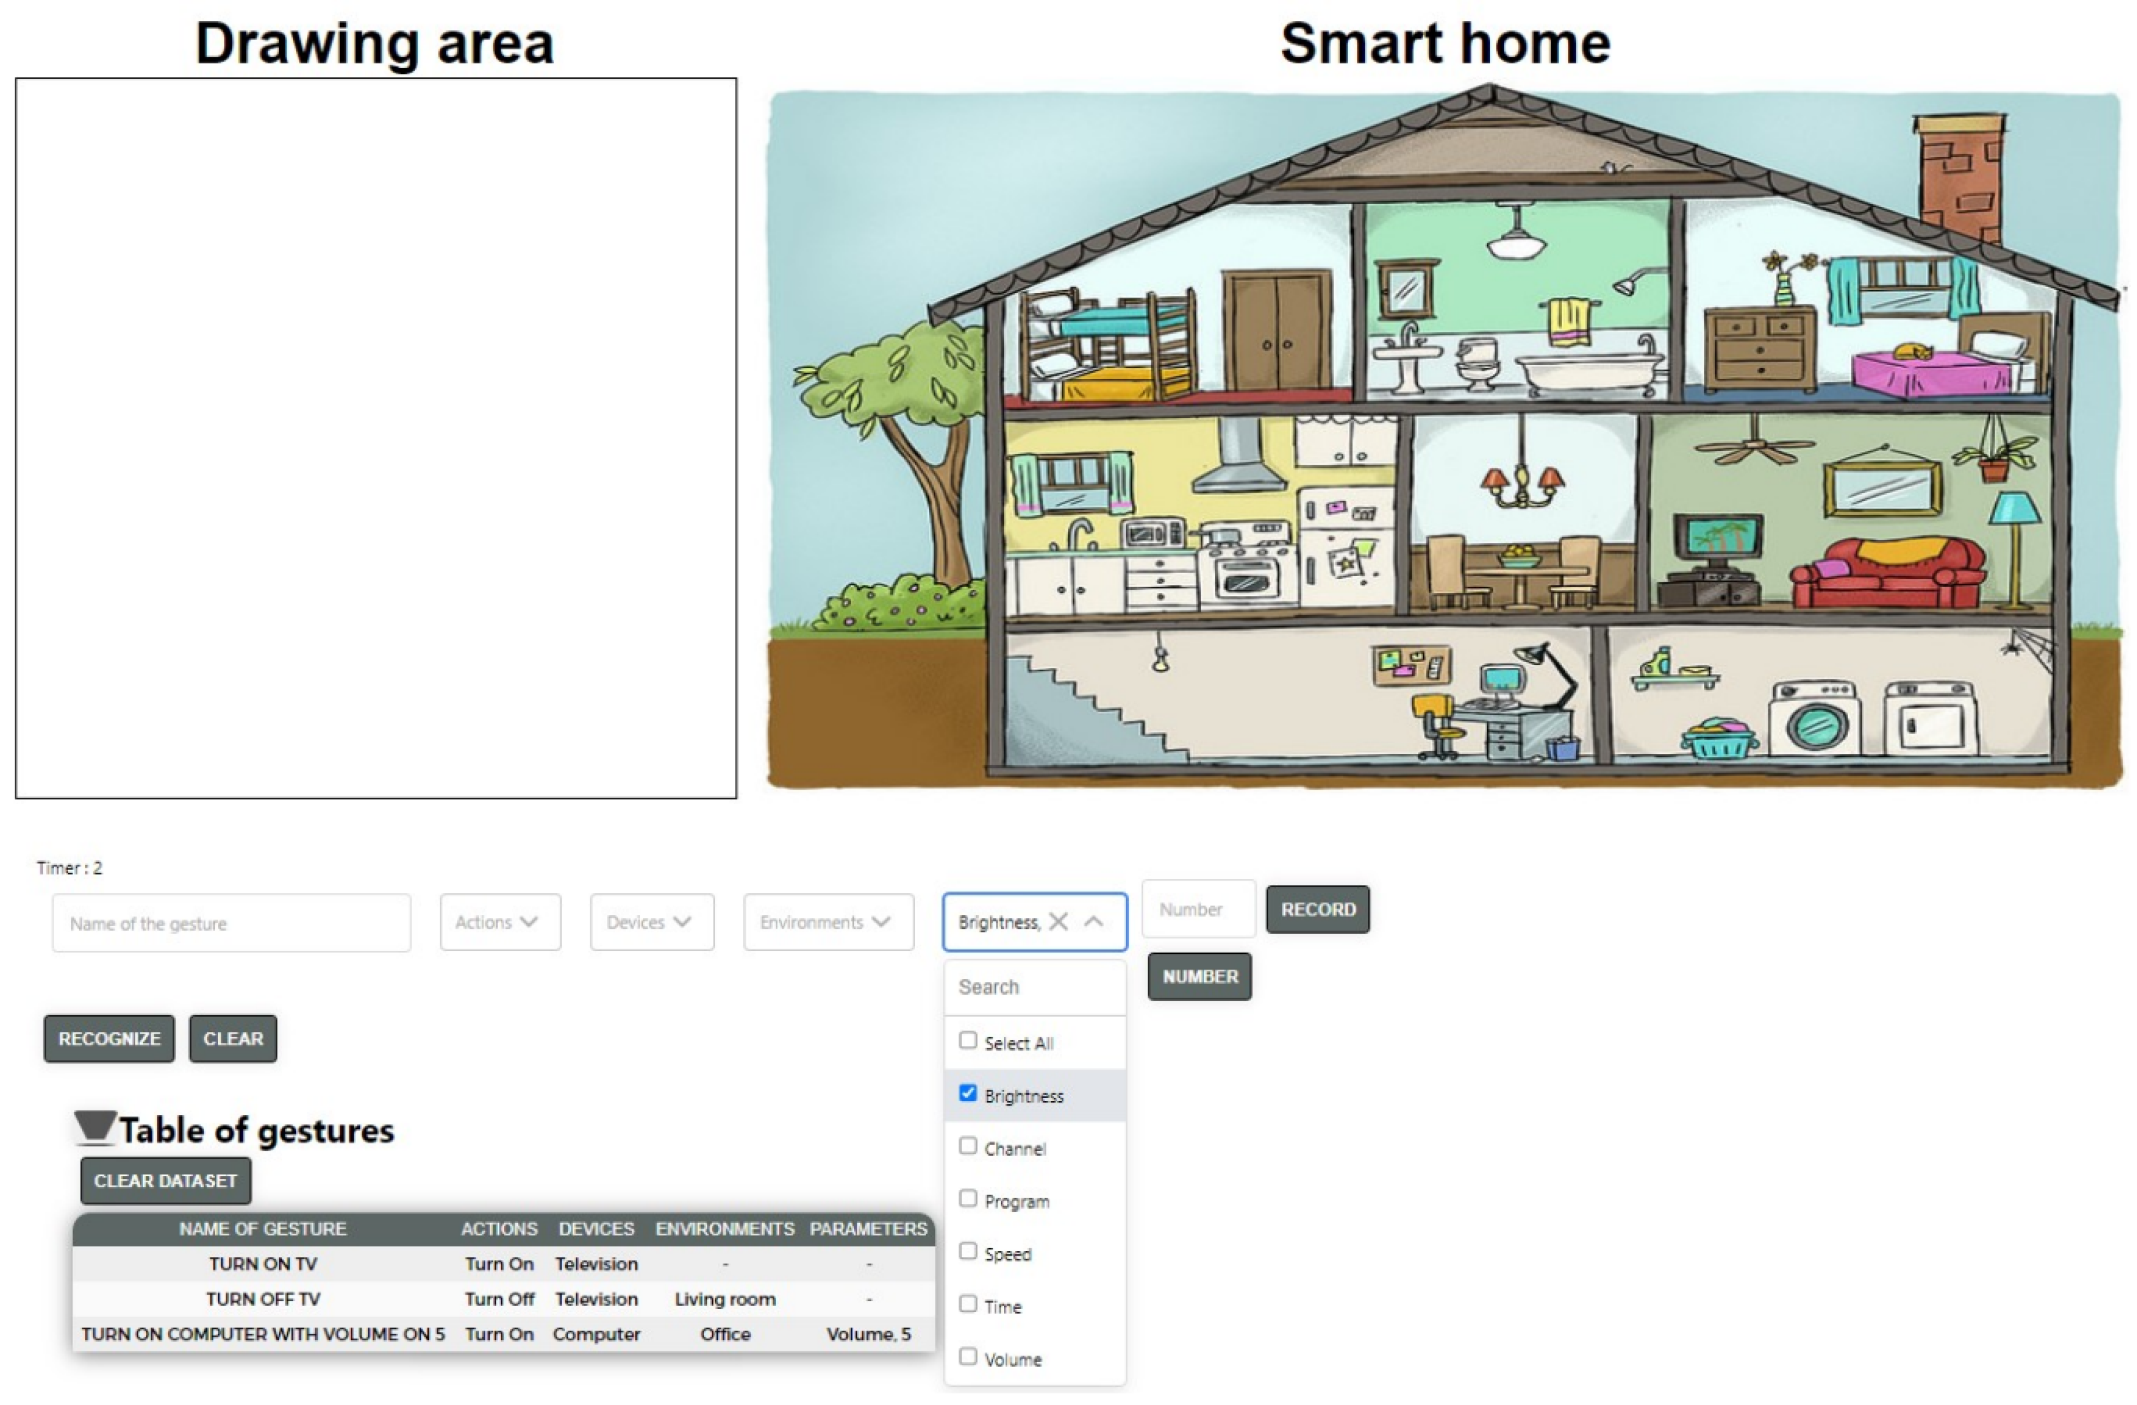
\includegraphics[width=\linewidth,trim={0.1cm 0.1cm 0.1cm 0.1cm},clip]{Figures/QuantumLeap/Applications/smart-home-prototype.pdf}  
        \vspace{-15pt}
        \captionsetup{width=.9\linewidth}
        \caption{Smart home application~\cite{Moinnet:2022}.}
        \label{fig:quantumleap:apps:smart-home}
    \end{subfigure}

    % \vspace{-8pt}
    \caption{Examples of applications created with \ql.}
    \label{fig:quantumleap:apps}
    % \vspace{-12pt}
\end{figure}


%================================================================================%
\section{Discussion} \label{sec:quantumleap:discussion}
In this section, we discuss the main strengths and limitations of the \ql framework.

%--------------------------------------------------------------------------------%
\subsection{Strengths} \label{sec:quantumleap:discussion:strengths}
The modular approach to gesture recognition promoted by \ql offers many advantages compared to typical non-reusable and/or opportunistic approaches. 
%
First, \ql provides a clear separation of concerns between the UI design and the gesture recognition dataflow, which greatly facilitates updates to the UI, the supported set of gestures, and the dataflow. This separation of concerns also allows developers to ignore the specifics of gesture recognition when working on the application, thus lowering the barriers to entry into gesture-based UI development.
%
In addition, the standardized modules and datasets supported by \ql enable researchers and practitioners to efficiently reuse them across applications, share them, and seamlessly replace one module with another in a dataflow, \eg to improve performance.
%
Finally, the \ql GUI allows developers to visualize and change the settings of the dataflow and its modules in a few clicks without having to access and modify their source code. Dataflow configurations can be exported from the GUI and shared with other researchers and practitioners.

%--------------------------------------------------------------------------------%
\subsection{Limitations} \label{sec:quantumleap:discussion:limitations}
There is, however, still plenty of room for improvement.
%
First, the \ql GUI only provides limited guidance, in the form of short textual descriptions of modules and settings, for configuring the gesture recognition dataflow (Section~\ref{sec:quantumleap:description:configuration}). As such, while \ql reduces the effort required for developing gesture-based applications, some understanding of the modules (\eg gesture recognizers) is still required to build an efficient dataflow.
%
In addition, the dataflow architecture of \ql combines modularity with some rigidity. For instance, supporting more than one user, adding new module types (\eg a third type of gesture recognizer), or changing their order in the dataflow cannot be done easily without modifying the source code of the framework. This rigidity makes the framework more accessible to less experienced developers but may prevent some developers from experimenting with more advanced gesture recognition techniques.
%
Finally, \ql can only support one application at a time. Switching between two gesture-based applications thus requires users to manually switch their configurations within the \ql GUI and restart the framework.

%================================================================================%
\section{Conclusion} \label{sec:quantumleap:conclusion}
% Summary
In this chapter, we introduced \ql, a framework for engineering gestural user interfaces based on the Leap Motion Controller by leveraging several barriers encountered in the development life cycle of gesture-based interactive applications. To facilitate the development of such LMC gesture-based UIs, manual development is replaced by configuring existing modules implemented in \ql in a dataflow way that can be saved in a configuration file for future usage.
%
We demonstrated its usability in an experiment with seven participants of varying levels of expertise and showcased different use cases of \ql proposed by students and colleagues throughout the years. They actively contributed to the project by implementing new modules and crafting unique gesture-based applications.

% Software quality properties
We remained mindful of the four software quality properties mentioned in Section~\ref{sec:introduction:research:research-questions} throughout the design and development of \ql.
%
Regarding \textit{compatibility}, the standardized modules and datasets of \ql can be seamlessly shared and reused across applications. In particular, these components are interoperable with the testing tool described in Chapter~\ref{chap:quantumleap-testing}. This interoperability would extend in the future to other applications and tools that use the same dataset format and module interfaces.
%
From a \textit{maintainability} perspective, updates to a module are isolated, thus minimizing the impact on other modules. The clear separation of concerns between an application and its gesture recognition logic further enables developers to modify the dataflow without altering its application code. It also provides the flexibility to transition to a different framework than \ql, should a more suitable alternating become available. 
%
In terms of \textit{portability}, \ql configurations, modules, and datasets can be reused in other applications. Moreover, modules and datasets used in a dataflow can be replaced to support a different environment in a matter of seconds with minimal impact on applications, requiring only a quick restart of the dataflow. 
%
As for \textit{usability}, leveraging \ql enables developers to prioritize user experience instead of spending time to implement gesture recognition from scratch. In addition, applications built with \ql can also easily accommodate user-defined gestures, resulting in enhanced usability~\cite{Nacenta:2013}.

% Future works
Future work can be envisioned at increasing levels of granularity. 
%
At the framework itself, improvements could focus on three key aspects.
%
First, we could refine the architecture of \ql, introducing greater flexibility to accommodate more complex dataflows. Changes could include supporting gestures from multiple users simultaneously, changing the order of modules in the dataflow, or integrating custom module types.
%
Enhancing the flexibility of \ql would also increase its complexity. As such, it will be essential to provide more guidance to developers when configuring the dataflow, \eg by automatically suggesting suitable configurations based on the selected sensor(s) and gesture set.
%
In addition, we could enable applications to submit their dataflow configuration upon connecting to \ql, automatically downloading missing modules in the process. This feature would allow users to seamlessly switch between applications without having to manually change the configuration each time. In addition, this would enable users to replace default gestures with custom ones directly from within an application.
%
At a finer level (\ie the framework modules), future work could focus on gesture segmentation, gesture recognition, and motion tracking sensors. We could explore novel methods for segmentation, such as Taranta \etal's work~\cite{Taranta:2017} which trains a recognizer with automatically generated examples of parasitic gestures to distinguish them from those that are intended by the user. Equally interesting is Leiva \etal's approach~\cite{Leiva:2018} that automatically generates synthetic gestures based on a template to train a recognizer, thus avoiding asking several participants to acquire gestures. In addition, we could study the impact of combining multiple sensors and/or gesture recognizers on recognition accuracy.